\chapter{Annotation~Experiments}
\label{chap:annotation} 

In this chapter I demonstrate the practical use of the annotation tool by annotating 10 different datasets. Representative images are shown in figure~\ref{fig:datasets_all}.



\section{Datasets}

\begin{figure*}[h!]
\centering
\begin{subfigure}[t]{0.24\linewidth}
  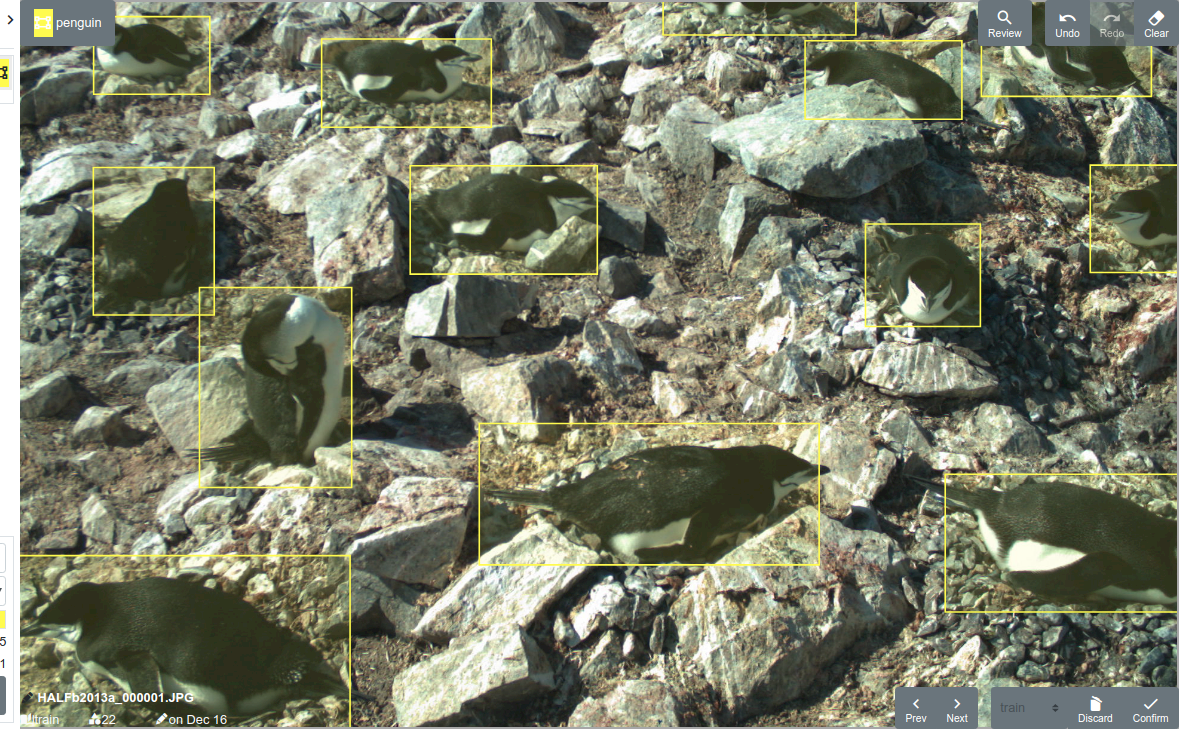
\includegraphics[width=1.0\linewidth]{figures/annotation/screenshots/penguins2.png}
   \caption{\emph{penguins}}
\end{subfigure}%
\begin{subfigure}[t]{0.24\linewidth}
  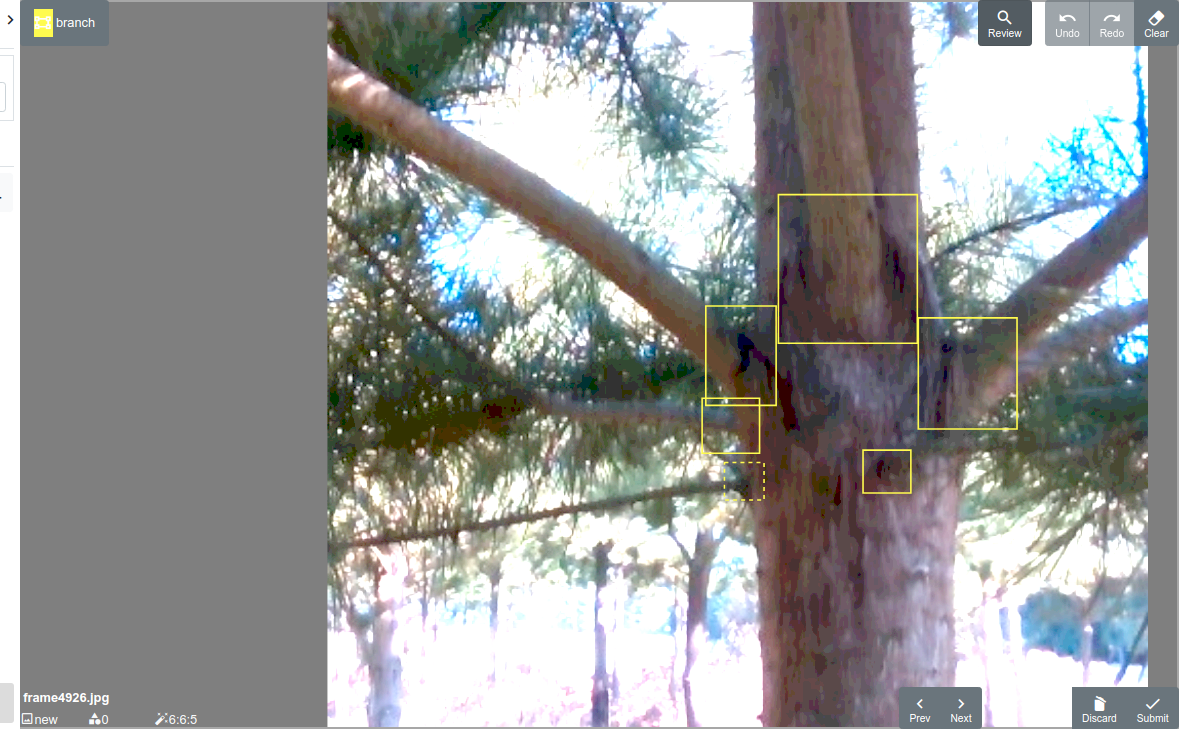
\includegraphics[width=1.0\linewidth]{figures/annotation/screenshots/branches3.png}
   \caption{\emph{branches}}
\end{subfigure}%
\begin{subfigure}[t]{0.24\linewidth}
  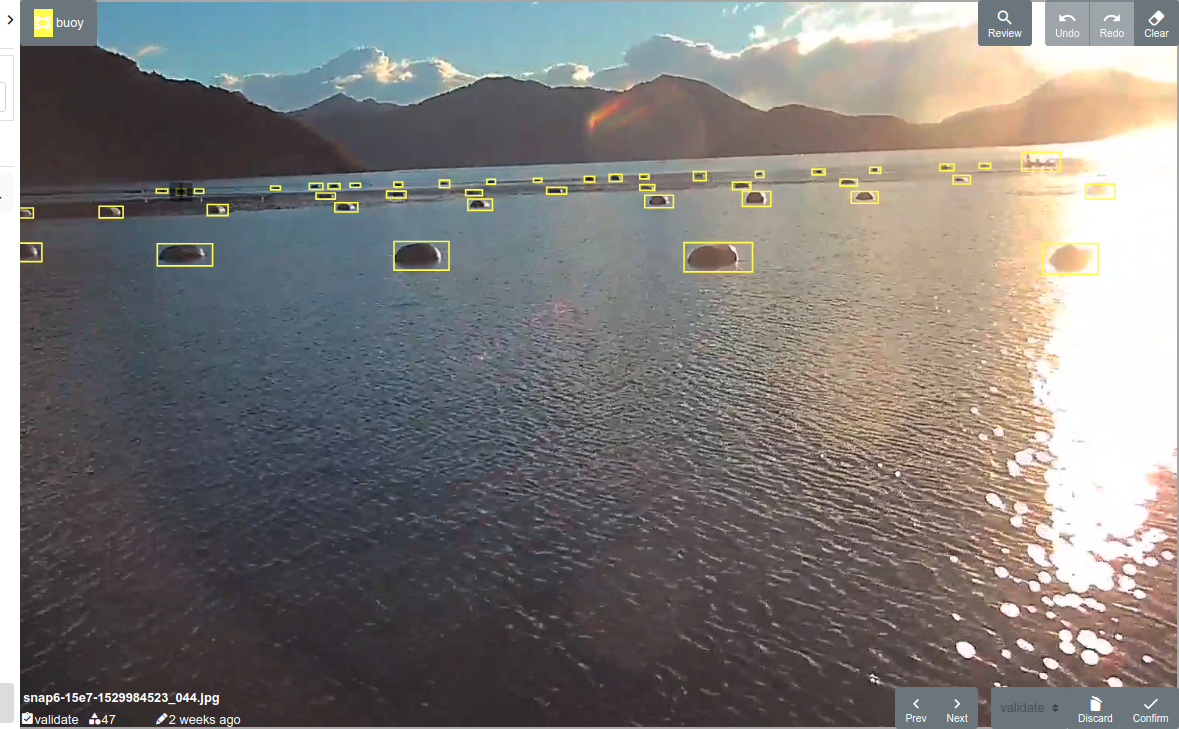
\includegraphics[width=1.0\linewidth]{figures/annotation/screenshots/buoys.png}
   \caption{\emph{buoys}}
 \end{subfigure}
\begin{subfigure}[t]{0.24\linewidth}
  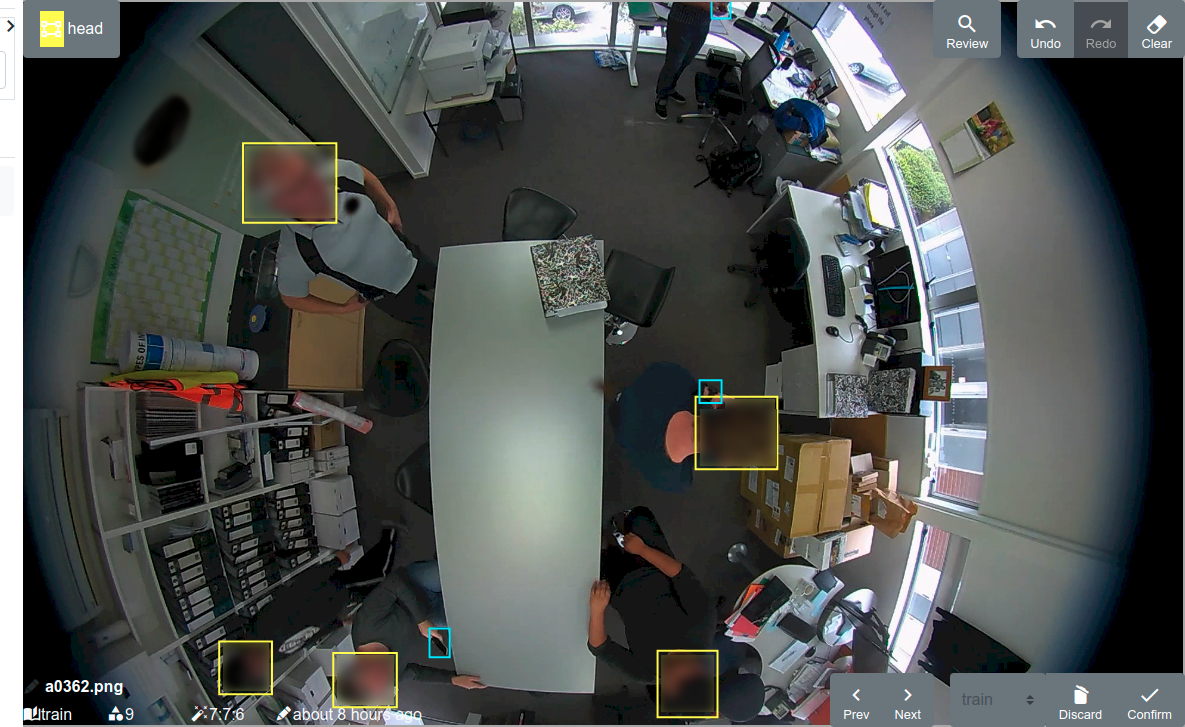
\includegraphics[width=1.0\linewidth]{figures/annotation/screenshots/victor.png}
  \caption{\emph{fisheye}}
\end{subfigure}%

\begin{subfigure}[t]{0.24\linewidth}
  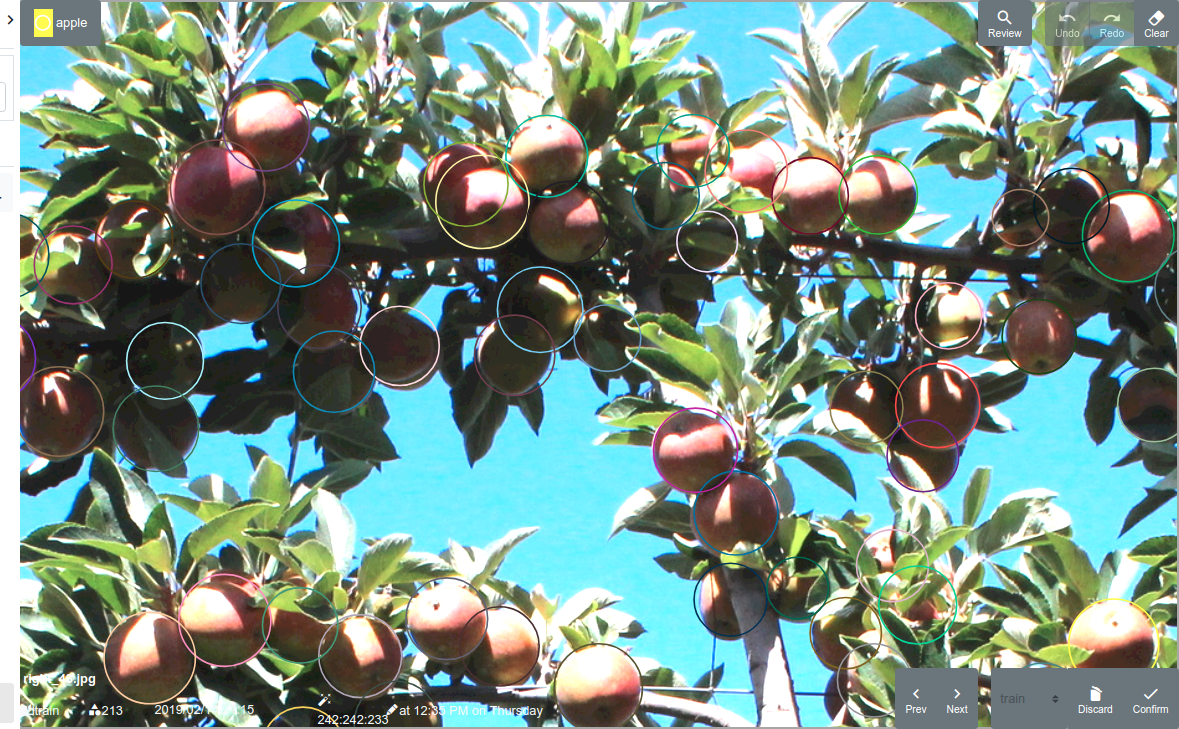
\includegraphics[width=1.0\linewidth]{figures/annotation/screenshots/apples_big2.png}
  \caption{\emph{apples}}
\end{subfigure}%
\begin{subfigure}[t]{0.24\linewidth}
  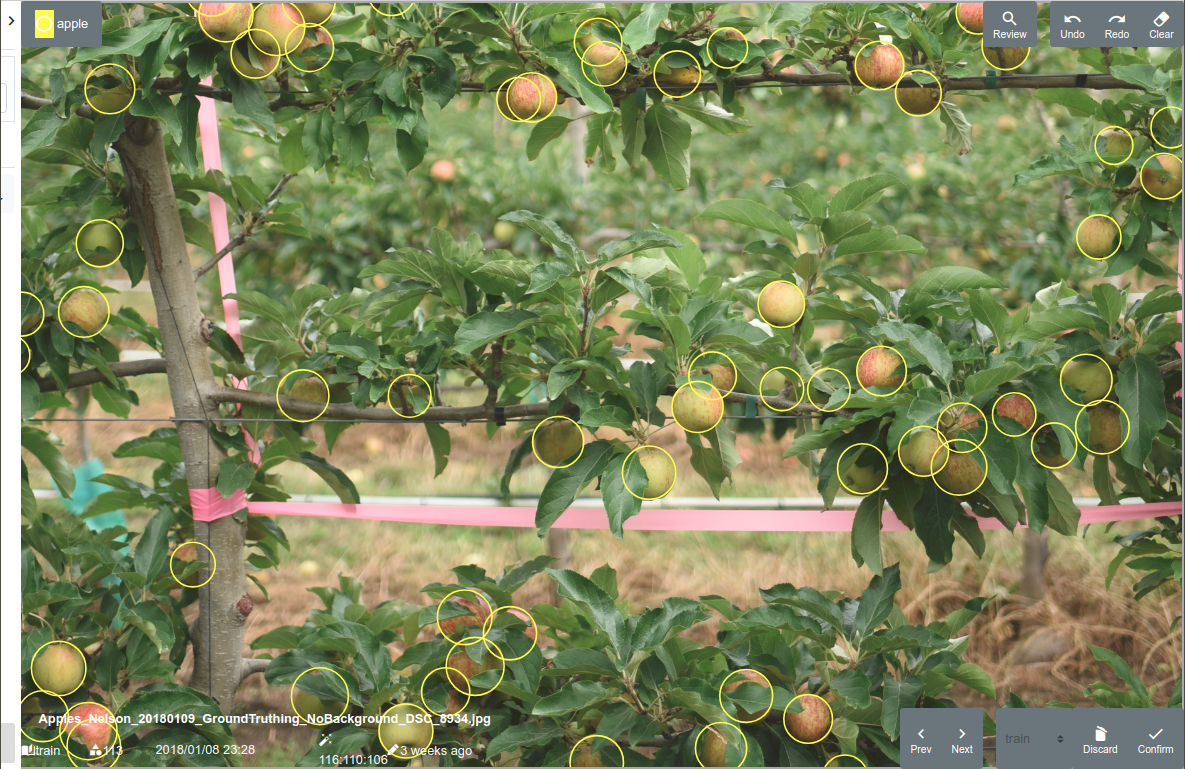
\includegraphics[width=1.0\linewidth]{figures/annotation/screenshots/apples2.png}
  \caption{\emph{apples2}}
\end{subfigure}%
 \begin{subfigure}[t]{0.24\linewidth}
  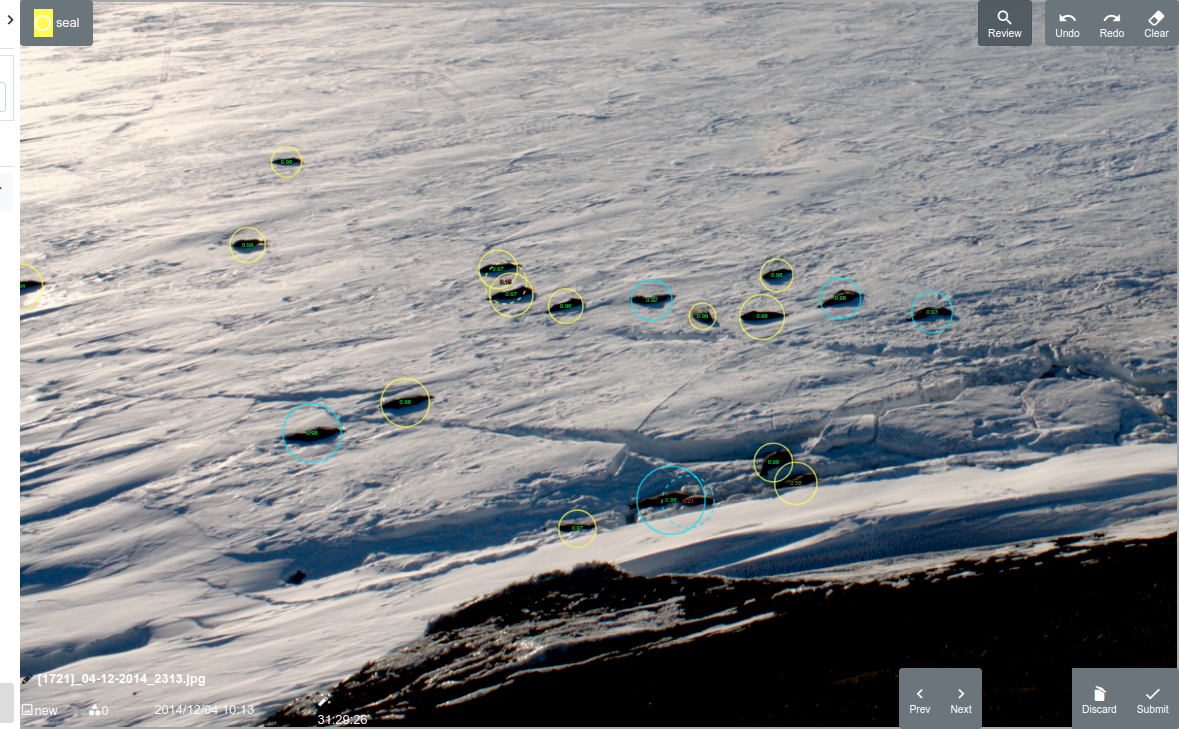
\includegraphics[width=1.0\linewidth]{figures/annotation/screenshots/seals_small2.png}
  \caption{\emph{seals}}
\end{subfigure}%
\begin{subfigure}[t]{0.24\linewidth}
  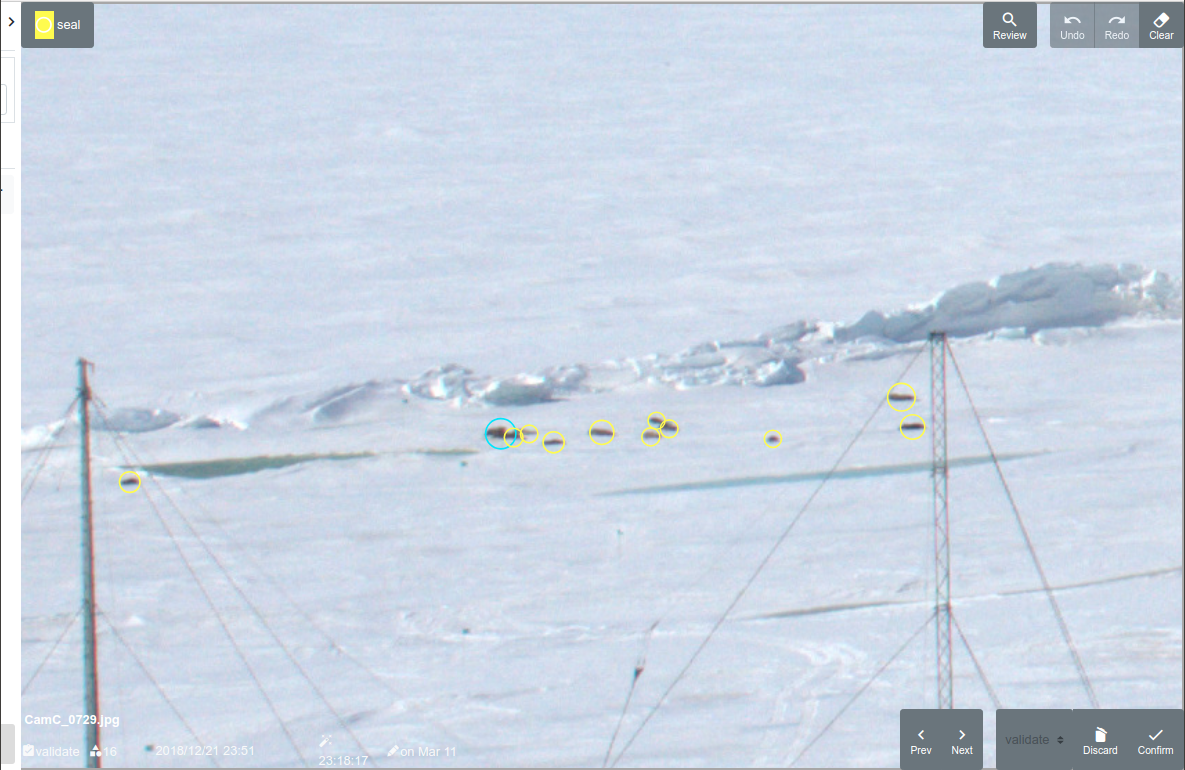
\includegraphics[width=1.0\linewidth]{figures/annotation/screenshots/scott_base_sunny.png}
  \caption{\emph{scott base}}
\end{subfigure}
\begin{subfigure}[t]{0.24\linewidth}
  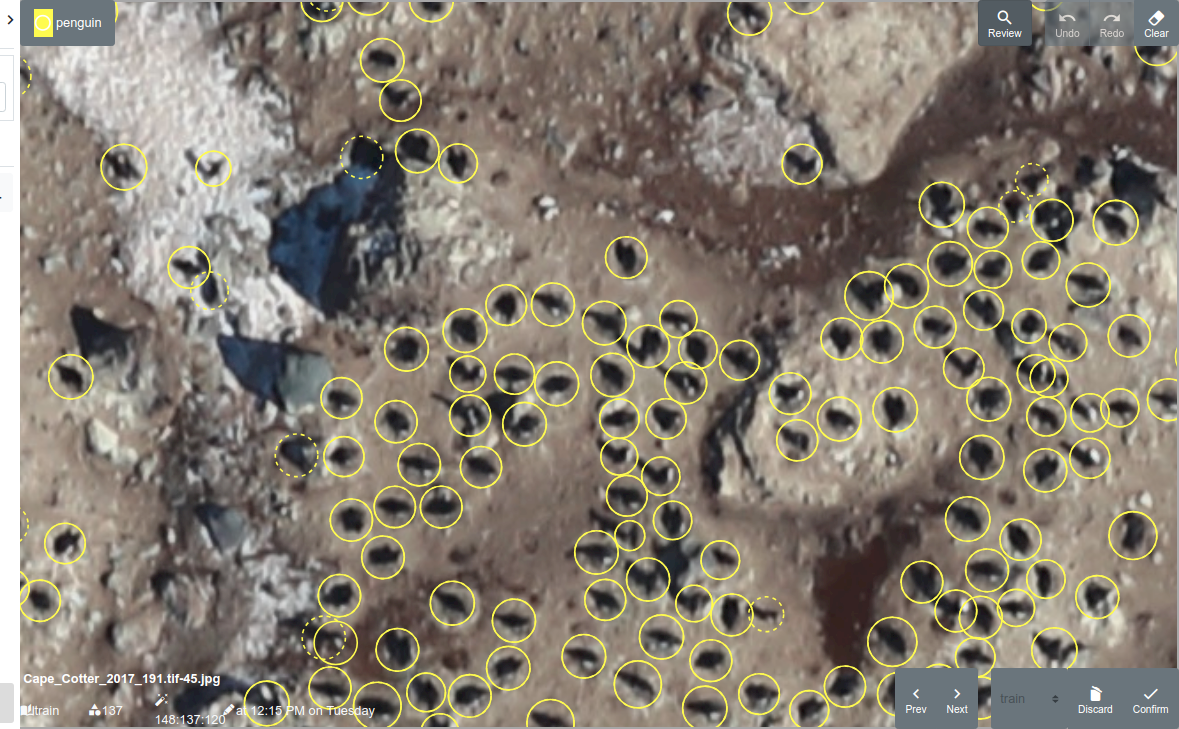
\includegraphics[width=1.0\linewidth]{figures/annotation/screenshots/penguins_aerial2.png}
  \caption{\emph{penguin survey}}
\end{subfigure}%
\begin{subfigure}[t]{0.24\linewidth}
  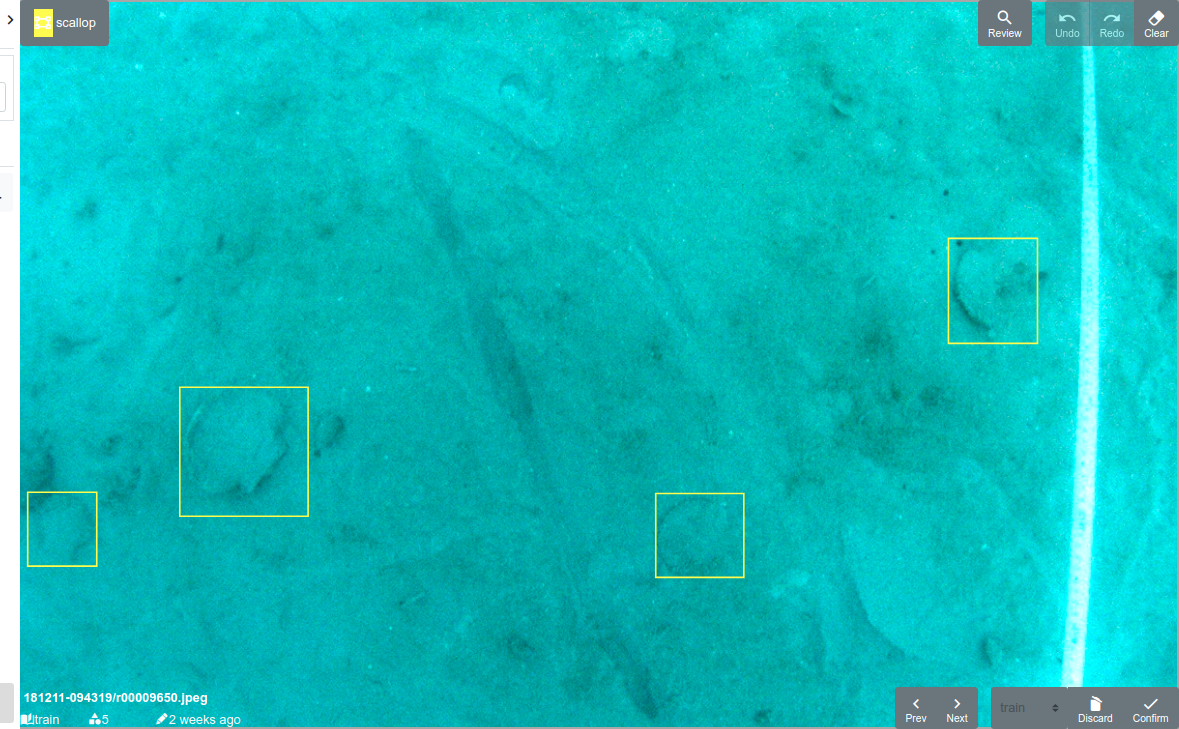
\includegraphics[width=1.0\linewidth]{figures/annotation/screenshots/scallops4.png}
  \caption{\emph{scallop}}
\end{subfigure}
 
\caption{Representative images of datasets (and annotations) annotated in this work}
\label{fig:datasets_all}
\end{figure*}

The datasets comprise a mix of relatively small scale image sets annotated for the sake of evaluating and developing the annotation method, image sets as test cases for future projects and a particular niche which seems suited to this kind of annotation method which is counting wildlife. In each case annotation time was between around an hour to around eight hours for the largest.

\begin{itemize}
    \item{\emph{penguins}}\par
A dataset used in the development of the annotation tool, primarily because the object detector performed well on the images after only a few annotated images and the relative uniformity of the images. The images used are a subset of the \emph{penguin dataset} \cite{PenguinData} used for counting using point annotations \cite{Arteta2016}. Originally these annotations were created from multiple people using the Zooniverse crowd sourcing platform \cite{Zooniverse}. 

Specifically the images annotated in this work (examples seen in figure~\ref{fig:penguin_dataset} were from the 'HALFb' subset, taken from a fixed camera position over a period of time. Many images in this dataset contain complex overlapping instances, however in the 'HALFb' there is a small amount of overlapping but for the most part the standard anchor box object detector has no trouble in detecting all of the instances.    
    \item{\emph{branches}}
    \item{\emph{buoys}}
    \item{\emph{fisheye}}
    \item{\emph{apples}}
    \item{\emph{apples2}}
    \item{\emph{seals}}
    \item{\emph{scott base}}
    \item{\emph{penguin survey}}
    \item{\emph{scallop}}
\end{itemize}



\section {Evaluation methods}
\label{sec:ann_evaluation}

The primary method of evaluation used in this work is that of \emph{continuous testing} whereby it is possible to characterise how the annotation process changes over time; how the model's predictions impact on the actions taken by the annotator, the type of actions and time required, and the accuracy of the model's predictions.

User edits are logged, along with predictions provided by the model (the starting point for annotating each image), and the final set of annotations submitted by the user. The accuracy of detections are verified directly by the user, giving both continuous testing of the model predictions as well as providing useful feedback to the user of the system. 

The types of actions as well as the timing can provide useful cues as to the difficulty of the task, and the level of assistance provided by the object detection model. 

I break down these actions, and the relation of the actions to the original set of detections and the performance of the object detector in a few different ways: categorise the action types and frequencies, categorise the corrections applied to each annotation, and lastly use a locally weighted \gls{AP} to quantify object detection performance on newly annotated images.

\subsection{User actions}

The various user actions are discussed in section~\ref{sec:user_interface} more detail. For the purposes of this chapter the user actions are broken down into categories:

\begin{itemize}
    \item {\bf transform}: an annotation is transformed (scaling, translation, corner dragged).
    \item {\bf confirm}: a weak detection is confirmed. This may also includes a transformation of bounding box, but as it is performed as one action.
    \item {\bf delete}: one or more annotations are deleted.
    \item {\bf add}: a new annotation is added.
    \item {\bf set class}: the class of an annotation is changed.    
    \item {\bf submit}: an image is submitted.    
\end{itemize}

\subsection{Annotation corrections}
\label{sec:corrections}

Another way of analysing the annotation process is to categorise each annotation by the nature of corrections applied to it (or used to create it) from predictions of the object detector. This differs from just looking at user actions because: (a) multiple actions may be performed on one annotation, for example, a scaling and a translation, or changing the class and translation (b) one action may modify multiple annotations, frequently a deletion of multiple false positives at once.

The following definitions are used:

\begin{itemize}
    \item {\bf positive}: a high confidence detection unchanged after verification.
    \item {\bf modified}: high confidence detection where either the box annotation or the class label has been modified.
    \item {\bf weak positive}: a weak detection confirmed translated).    
    \item {\bf false negative}: an object which was missed by the object detector and annotated manually by the user.    
    \item {\bf false positive}: an incorrect high confidence detection deleted by the user.
\end{itemize}

\subsection{Measuring progress with Cumulative Annotation Time}
\label{sec:ann_time}

\begin{figure}
\centering
  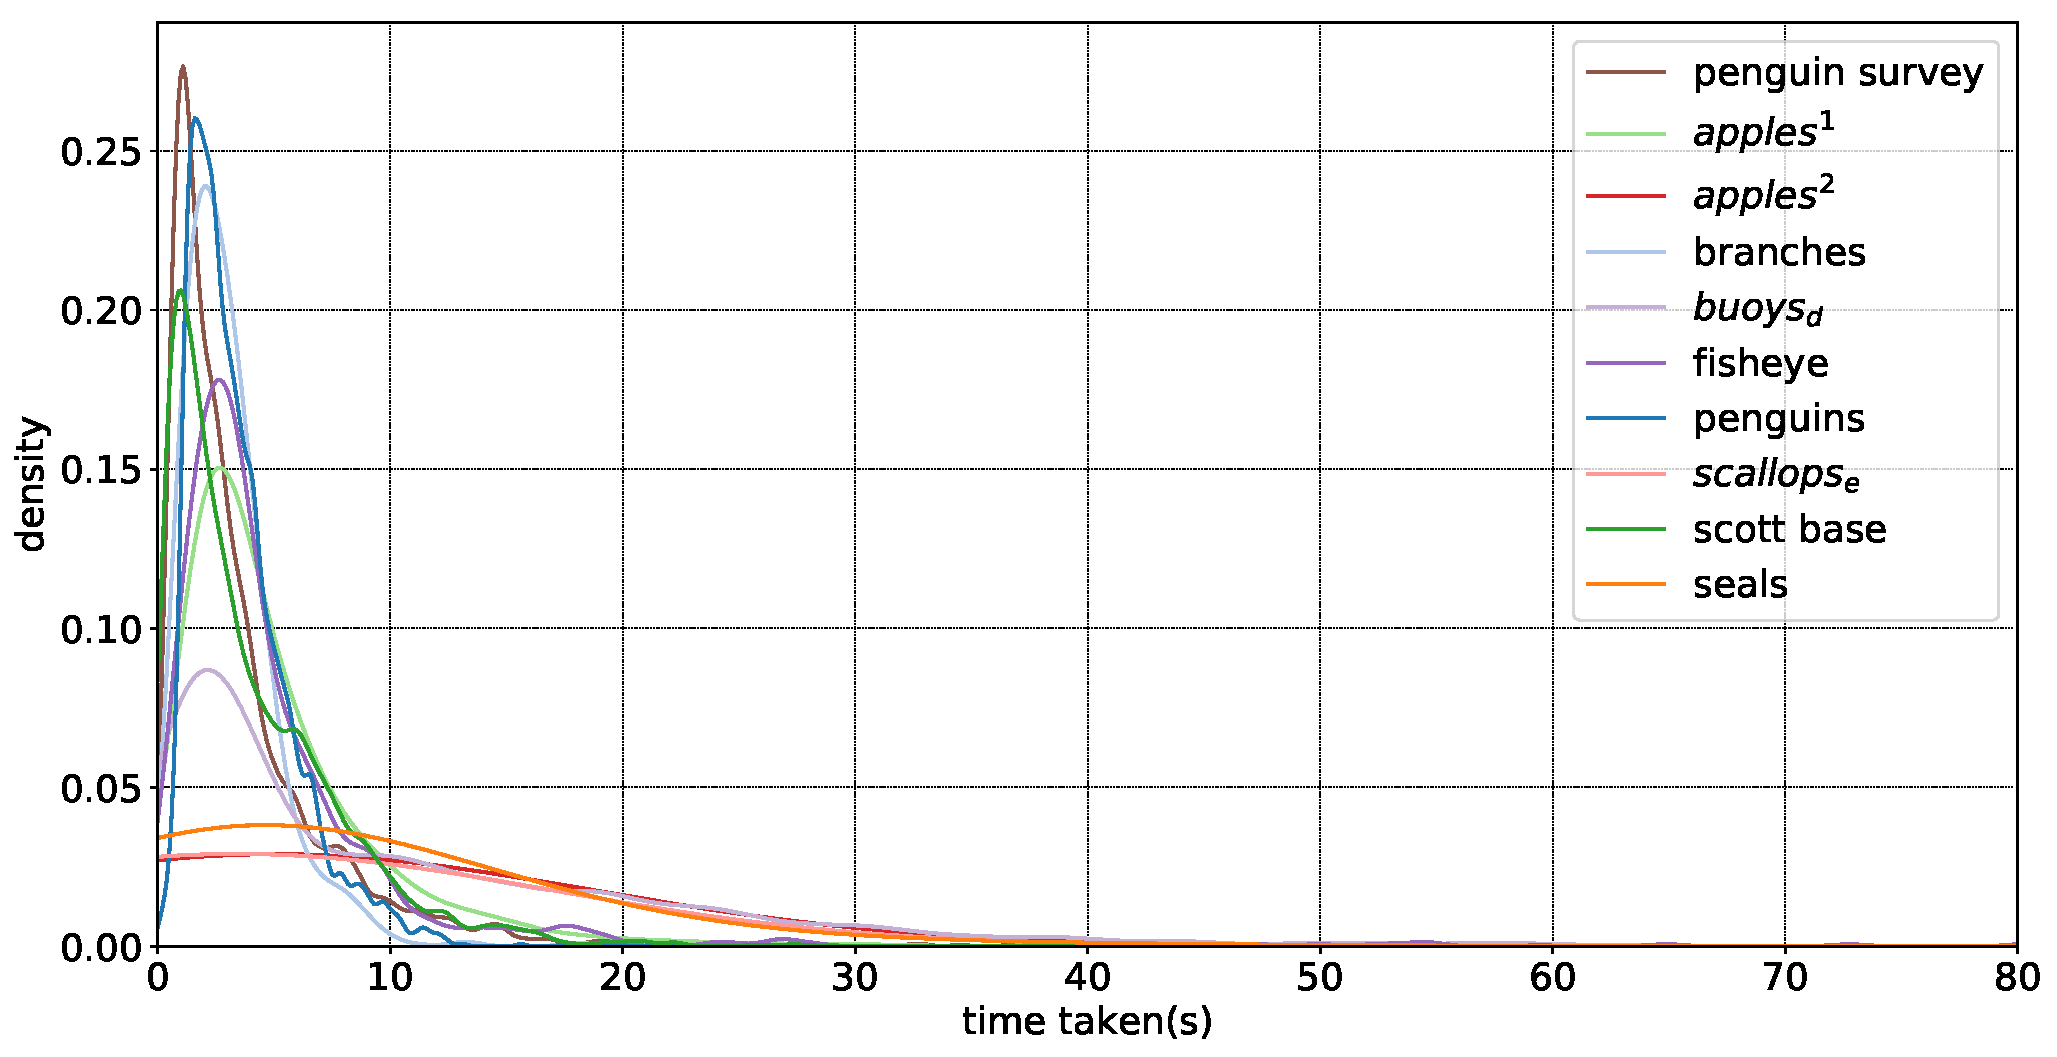
\includegraphics[width=1.0\linewidth]{charts/summaries/time_density.pdf}
  \caption{Time per action distributions for different dataset annotation}
  \label{fig:annotation_time_density}
\end{figure}

Measuring progress over the period of annotating a dataset. Due to the variation between images, the granularity of recorded annotations (often several hundred per image) the raw actions need to be grouped (for example, histograms over time). There are several ways progress could be measured in terms of annotation progress, such as the time spent since annotation began, the number of images or annotations submitted or the focus of this chapter, \gls{CAT} the total time the user spend has spent actively using the tool.

In section~\ref{sec:schedule}, trials incrementally enlarging the dataset showed the accuracy in validation to be strongly correlated to the number of examples used. For this reason we decide to use annotation progress (as opposed to training time for example) to visualise progress.

\subsection {Break detection}
\label{sec:break_detection}

The annotation logs recorded in this chapter were not taken in a controlled experimental setting, although an effort was taken to be consistent in datasets annotated by the author. Datasets annotated by others' can be seen to have more variability. It was therefore necessary to detect breaks where annotation was paused mid-image. Any action was capped at a maximum one minute for this purpose. Ideally this would have been detected directly in the tool by detecting lack of input or loss of focus, and future studies will take this approach. 

Figure~\ref{fig:annotation_time_density} shows the distribution of times per action for different annotation efforts where any action taking more than a minute is a significant outlier in most cases. An obvious discrepancy can be seen between the \emph{scott base}, \emph{seals} and \emph{scallop} datasets, this is because the video sequences are useful in resolving ambiguity and more time is spent looking forward and backward at previous frames.

\subsection{Visualisation}
\label{sec:visualisation}

In order to visualise trends in the user action types a fixed size density estimation is used with gaussian kernel, $\sigma=5 minutes$. This approach is taken for both user actions, annotation correction types, the rate of annotations and using a weighted \gls{AP} to quantify overall detector performance at a particular point in  time.

Annotation actions, corrected annotation types are all deemed to occur at the \gls{CAT} the image is submitted. Even though actions occurred at distinct points during an image annotation, the interest is in overall trends rather than particular trends within annotating each image. 

\subsection {Locally weighted Average Precision}
\label{sec:noisy_trends}

To give a single metric for object detection performance where parts of a dataset are more important than others I use a weighted \gls{AP}. The object detector's predictions are compared against the users final annotations. A standard matching procedure is performed for all images (as opposed to tracking the user edits as in section~\ref{sec:corrections}).

In order to align with user actions across \gls{CAT}, a locally weighted \gls{AP} is used. To evaluate the locally weighted \gls{AP} at a particular point in cumulative annotation time, each image is given a weight according to it's time difference from the image \gls{CAT}. As above the gaussian kernel with $\sigma=5 minutes$ is used.

Annotations in each image are weighted by the image weight for the purposes of counting false positive, false negative and true positive counts. From there weighted precision and recall and \gls{AP} are computed exactly as normal. See section~\ref{sec:evaluation_metrics}.


\section {Dataset overview}
\subsection {Size distribution}

\begin{figure}[ht]
\centering
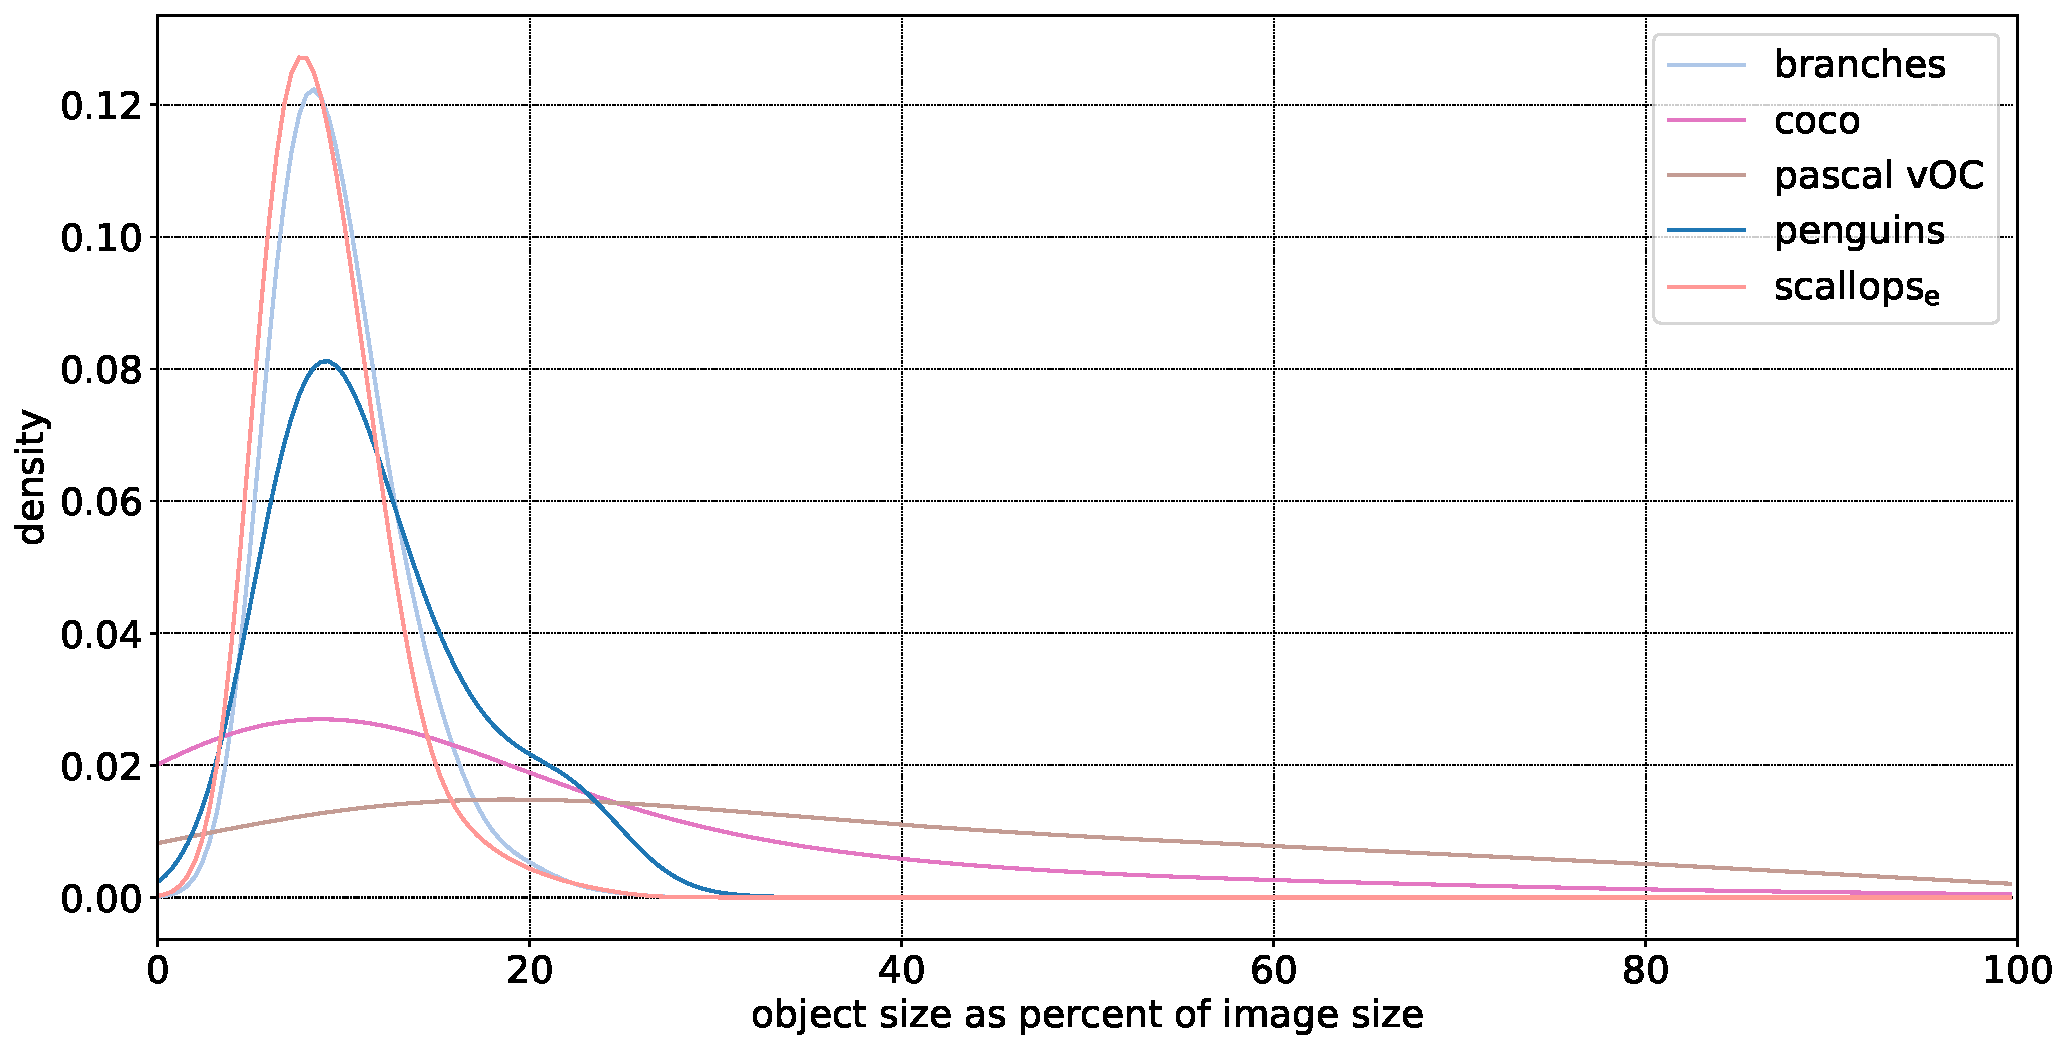
\includegraphics[width=1.0\linewidth]{charts/summaries/sizes_density.pdf}
\caption{Object bounding box size distributions as percent object to image size (average of width and height ratios) }
\label{fig:box_sizes}
\end{figure}


\begin{figure}[ht]
\centering
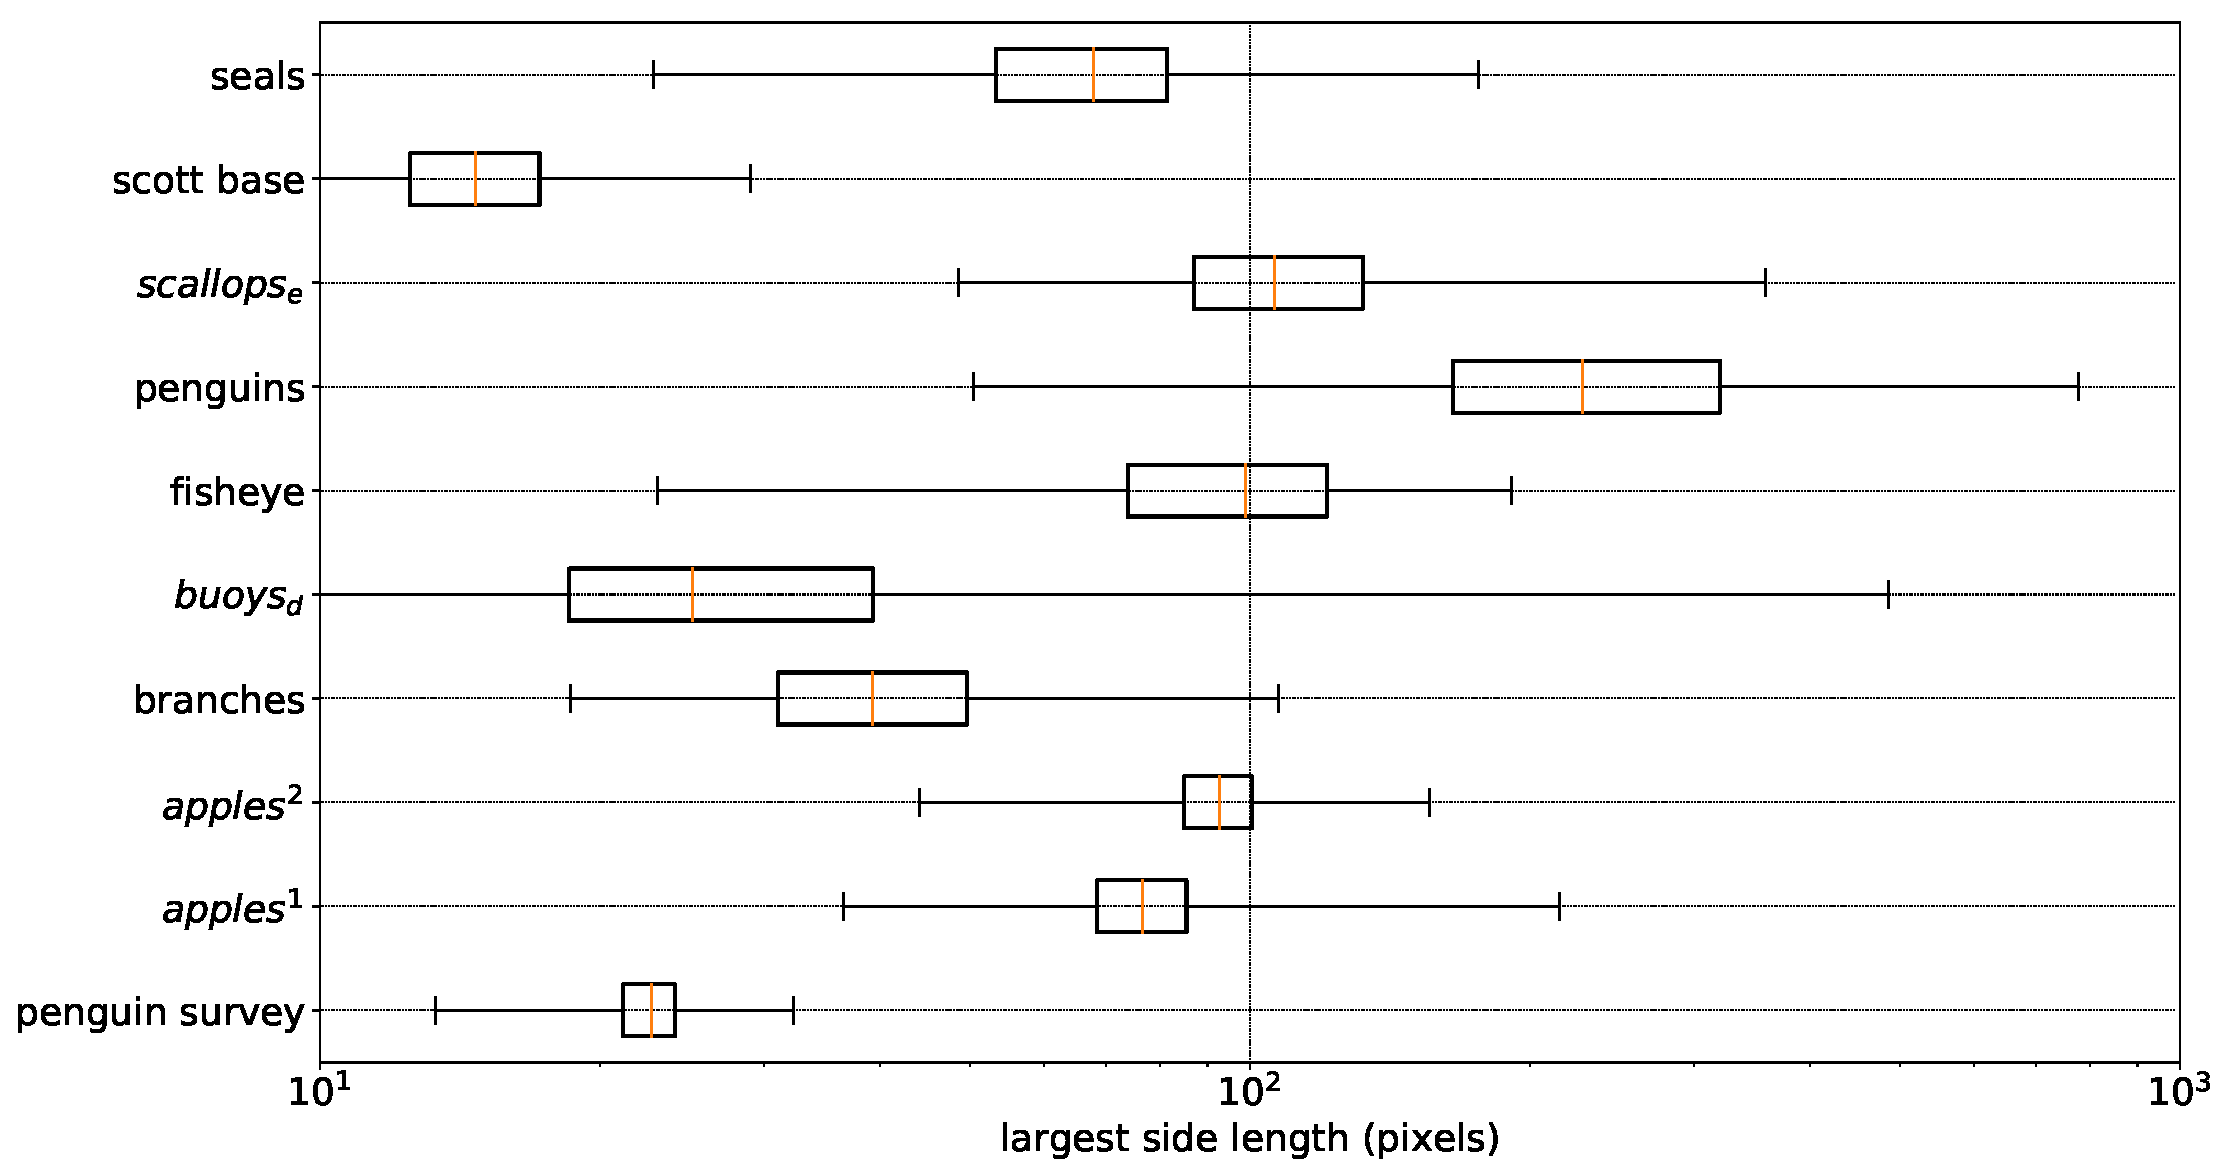
\includegraphics[width=1.0\linewidth]{charts/summaries/sizes_boxplot.pdf}
\caption{ Sizes in pixels of boxes for all annotated datasets }
\label{fig:box_sizes_plot}
\end{figure}

The sizes of objects in these datasets in general are small compared to more mainstream object detection datasets. This can be seen in figure~\ref{fig:box_sizes}, where compared to the Pascal VOC \cite{Everingham2008}, or COCO \cite{Lin2014}, the box sizes are smaller compared to the image size and less widely distributed. 

Figure \ref{fig:box_sizes_plot}  shows the object sizes (in pixels) of all the datasets together for comparison. In particular, the \emph{penguin survey} and \emph{scott base} datasets have particularly tiny objects (not shown on the figure in order to preserve the scale). It can be seen that although the box sizes are relatively small in terms of the relative size to the image that at full resolution the objects can be relatively large in pixels.

Two different types of annotations are used in the annotations of these datasets. Circular annotations are used for very small objects and for counting objects where precise localisation is of less concern; circular annotations are also used for apples where it just happens to match the object shape well. The difference to the object detector is little, instead of estimating two parameters, width and height it is simply a radius. In all other respects a circle is treated as a square for computations such as \gls{IOU} overlap.

\subsection {Instance distribution}

\begin{figure}[ht]
\centering
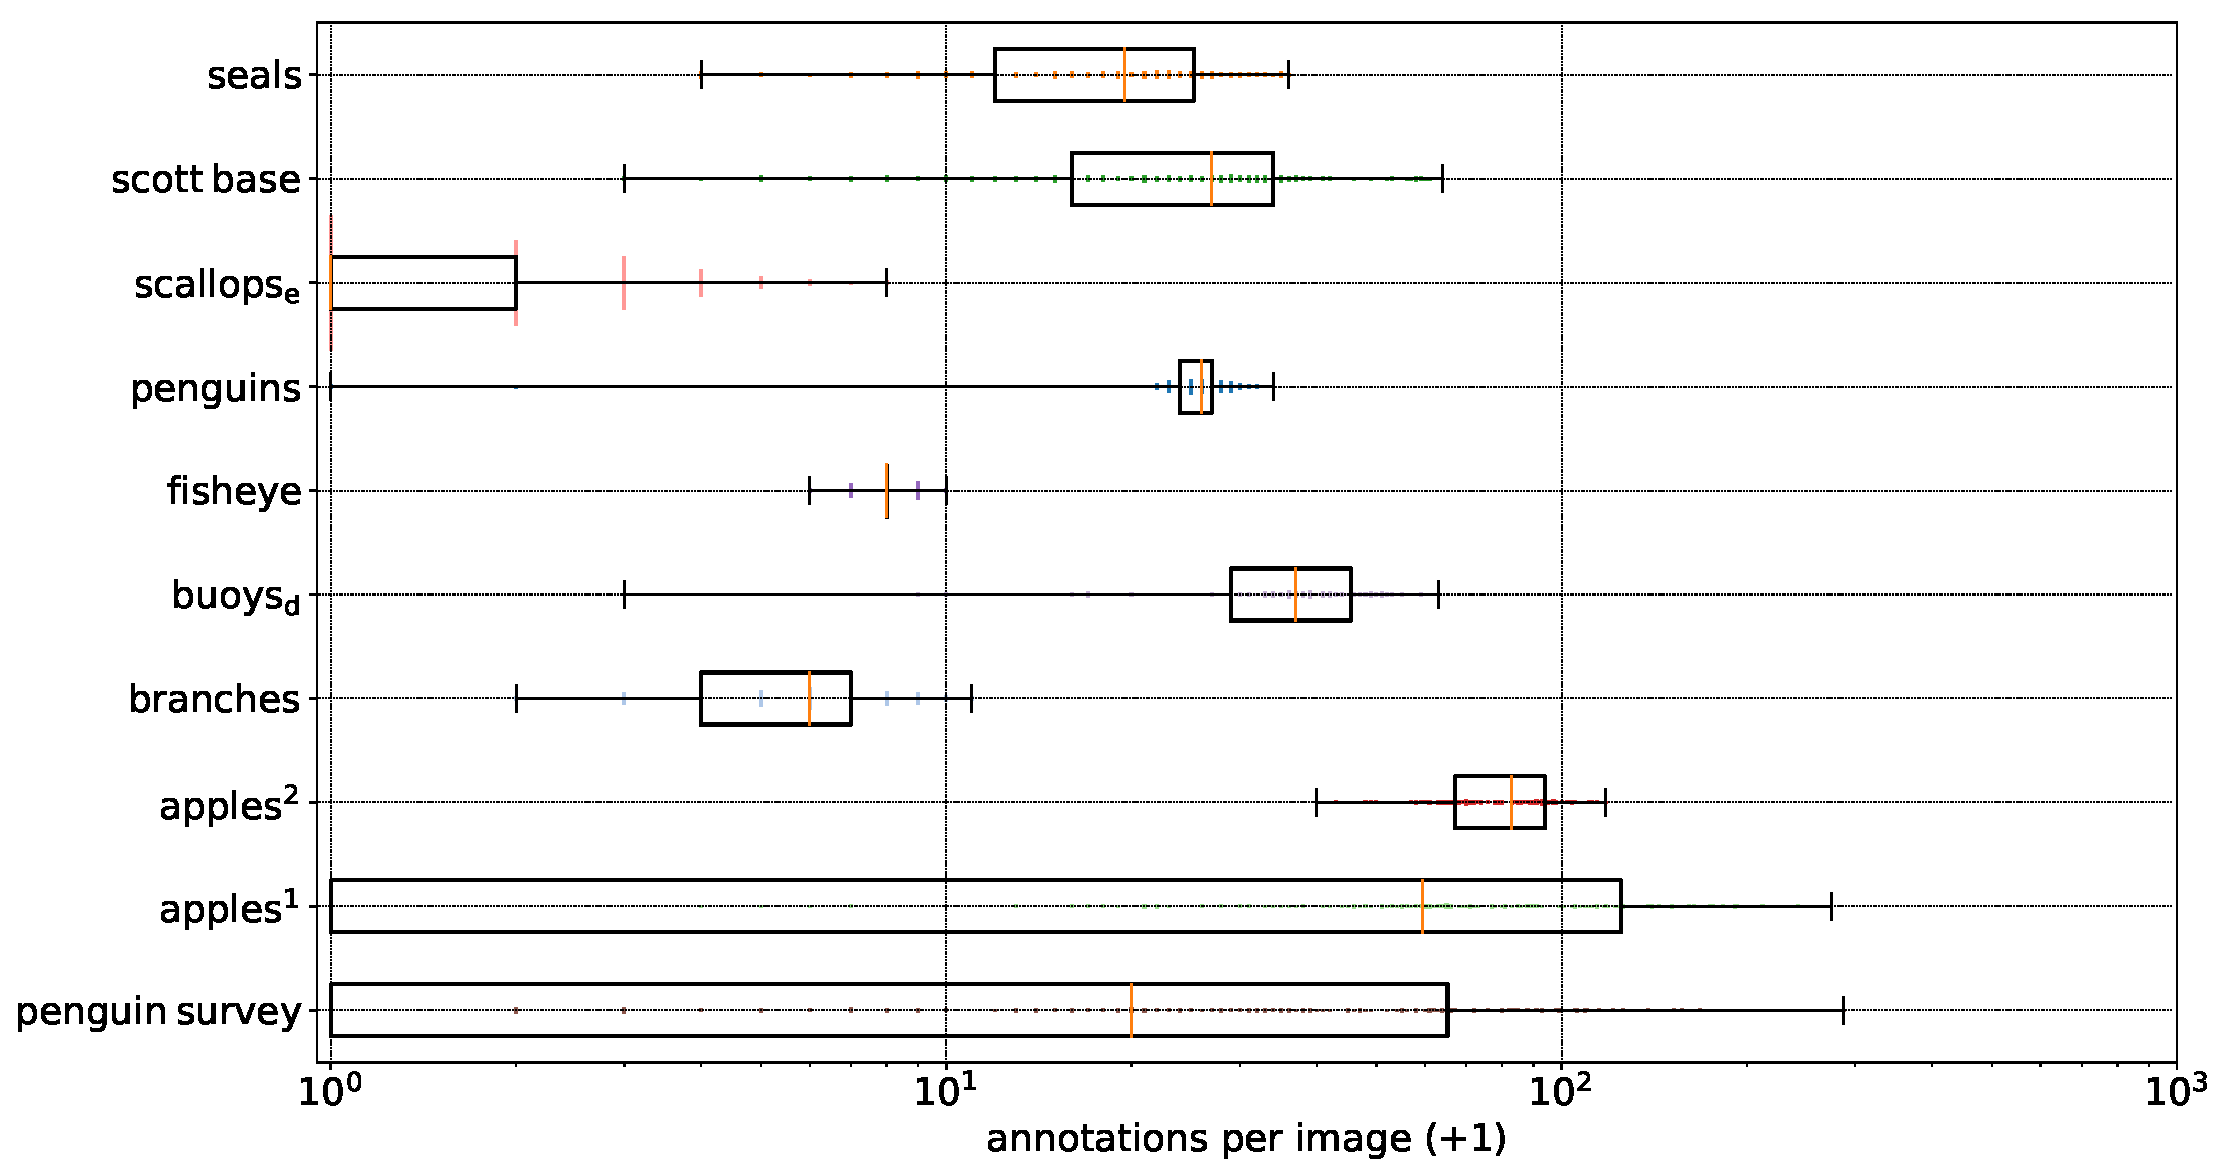
\includegraphics[width=1.0\linewidth]{charts/summaries/instances_boxplot.pdf}
\caption{ Distribution of object instances per image }
\label{fig:instances_image_plot}
\end{figure}

The datasets in question have a wide range of instance distributions, shown in figure~\ref{fig:instances_image_plot}. Some such as \emph{apples2}, \emph{branches} and \emph{fisheye} and \emph{penguins} contain a relatively uniform numbers of instances. Others especially \emph {penguin surveys}, \emph{scott base} and \emph{apples1} contain a wide range, a few with several hundred instances per image. One, \emph{scallops} contains very few instances and most images are negative images.


\subsection {Actions and corrections}

\begin{figure}[H] 
\centering
\begin{subfigure}{0.48\linewidth}
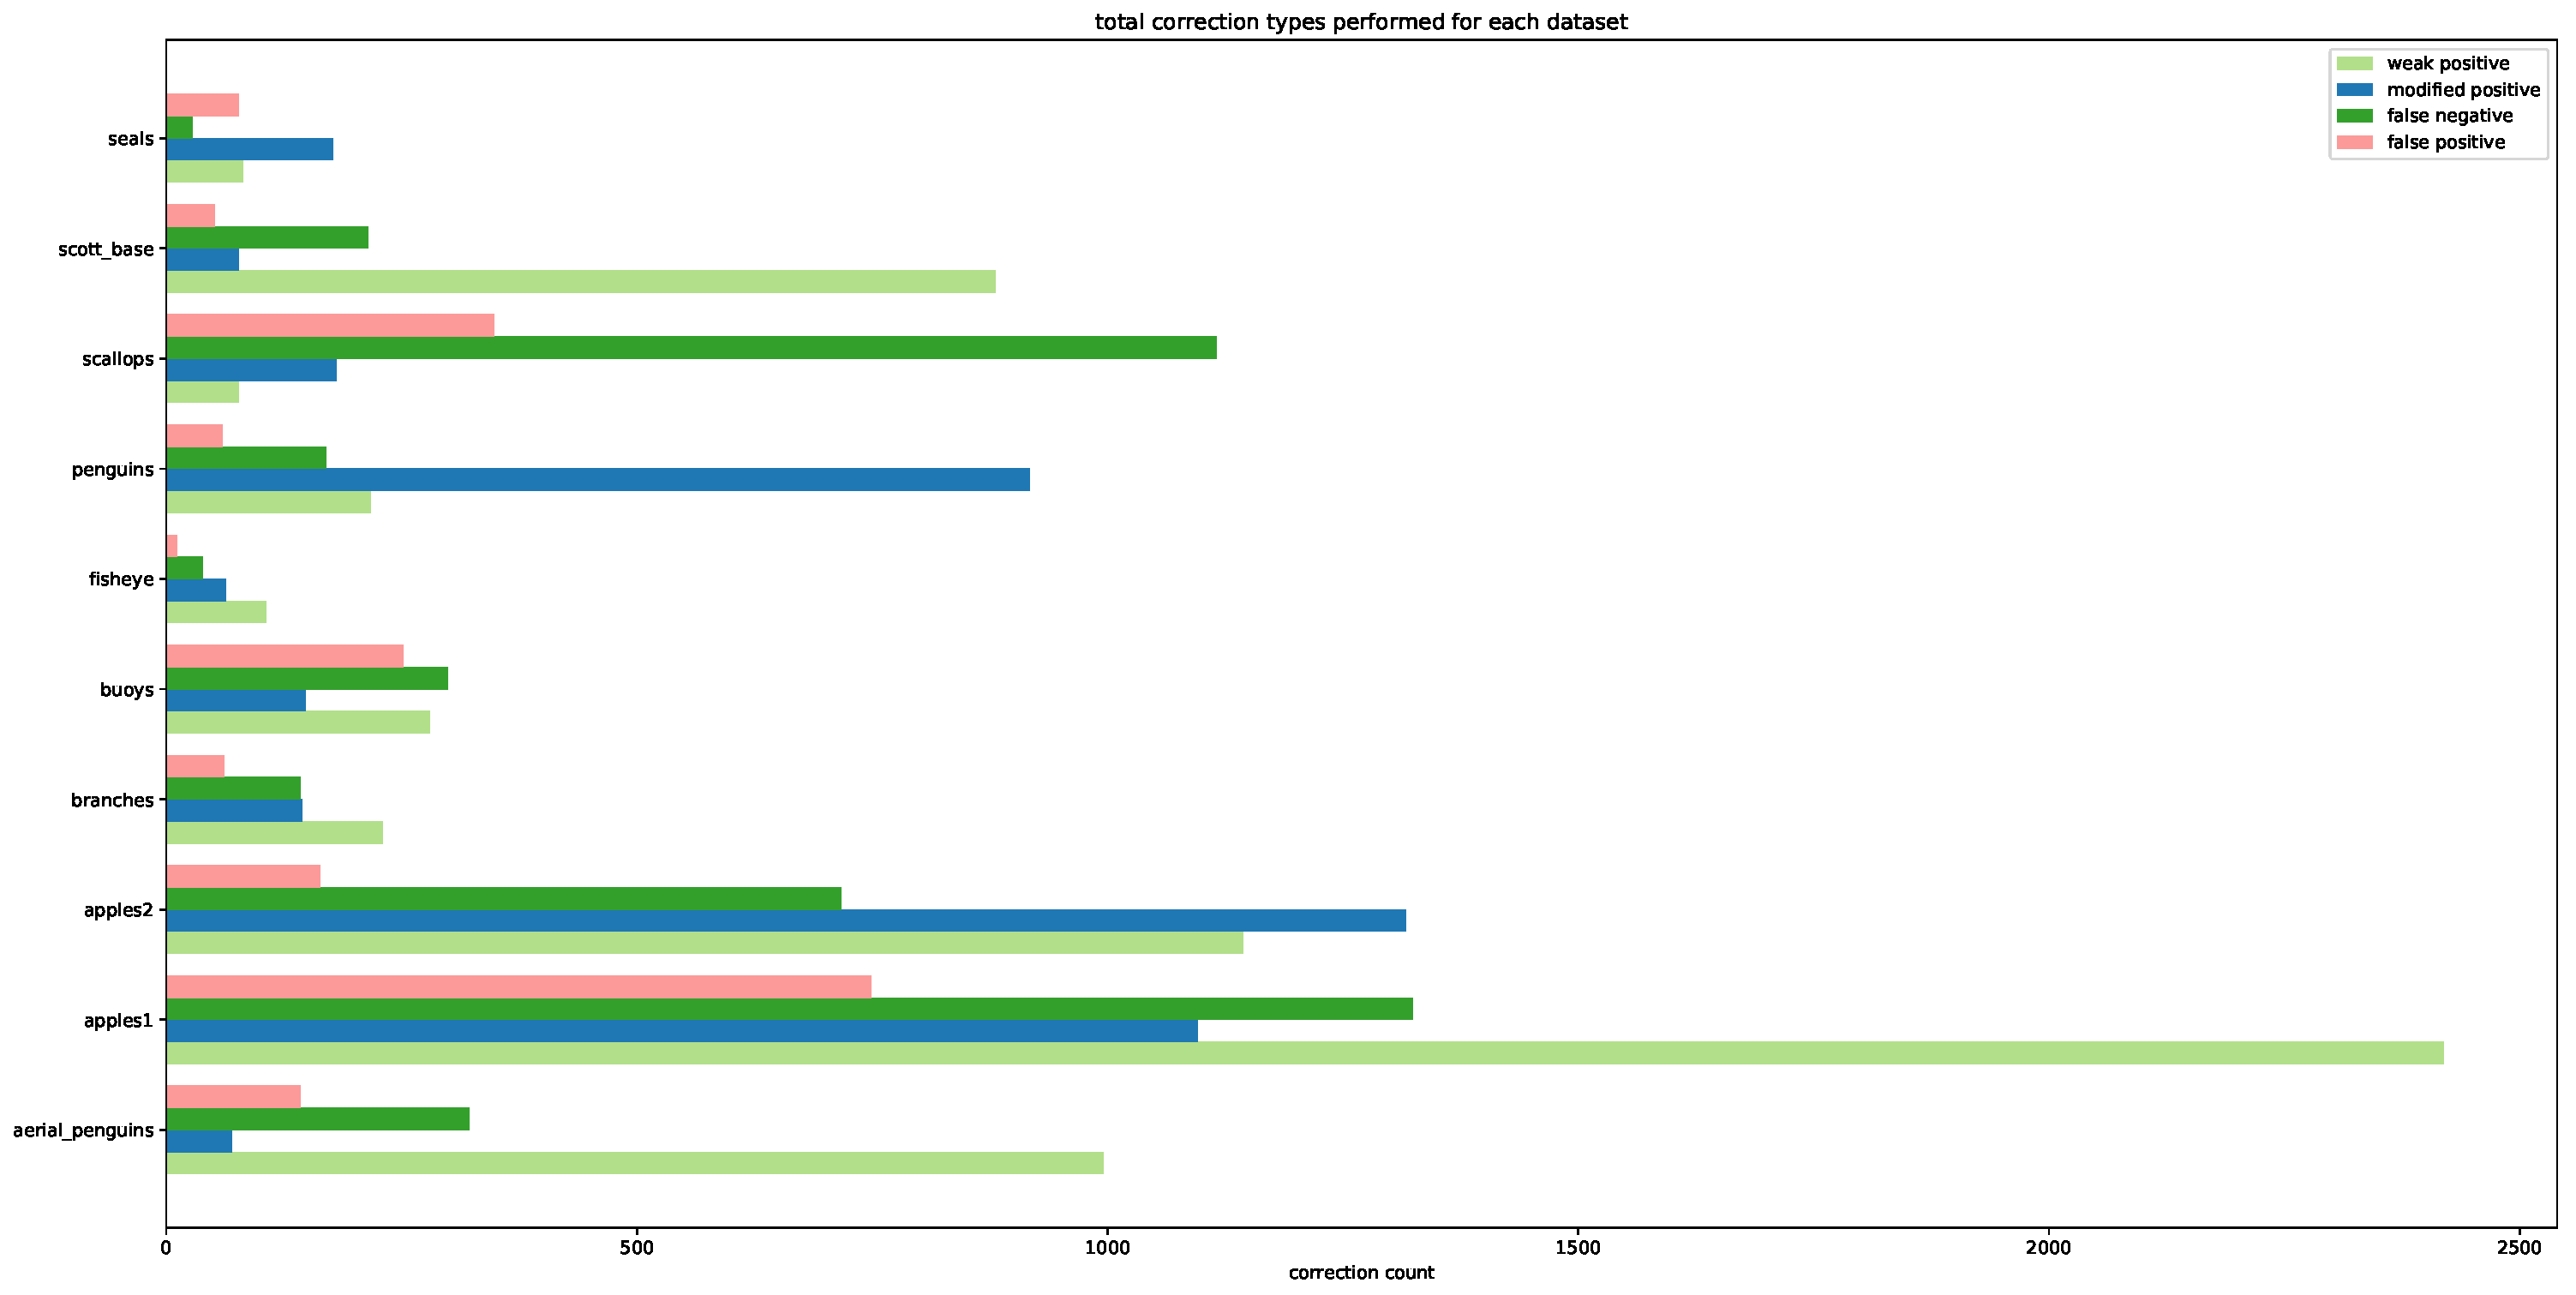
\includegraphics[width=1.0\linewidth]{charts/summaries/correction_counts.pdf}
\caption{Total corrections performed across datasets}
\end{subfigure}%
\begin{subfigure}{0.48\linewidth}
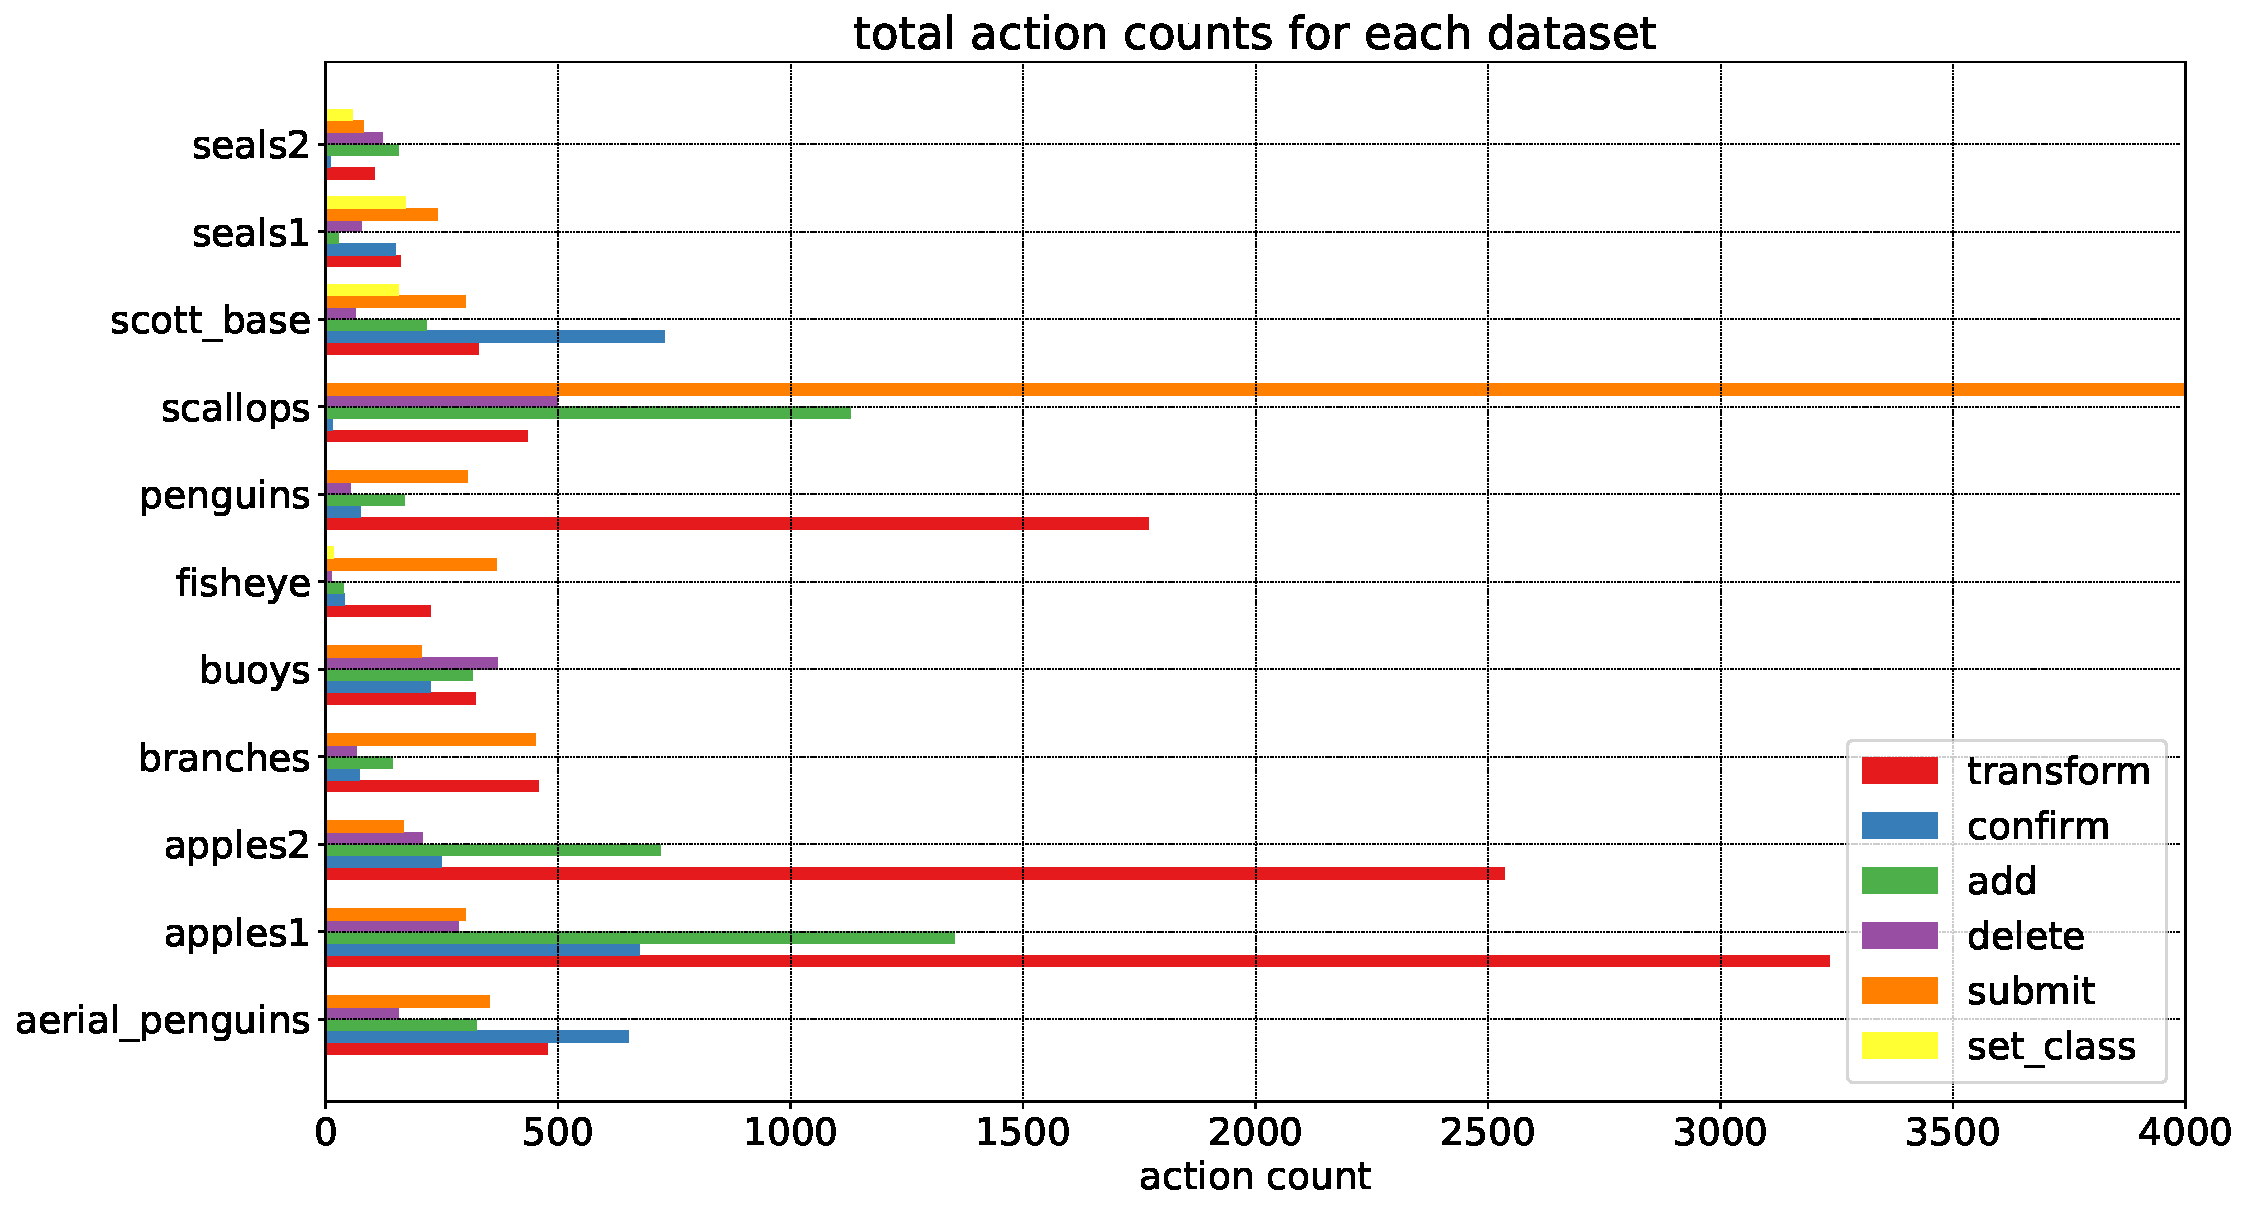
\includegraphics[width=1.0\linewidth]{charts/summaries/action_counts.pdf}
\caption{Total action counts across all datasets}
\end{subfigure}

\label{fig:actions_dataset}
\end{figure}



\begin{figure}[ht]
\centering
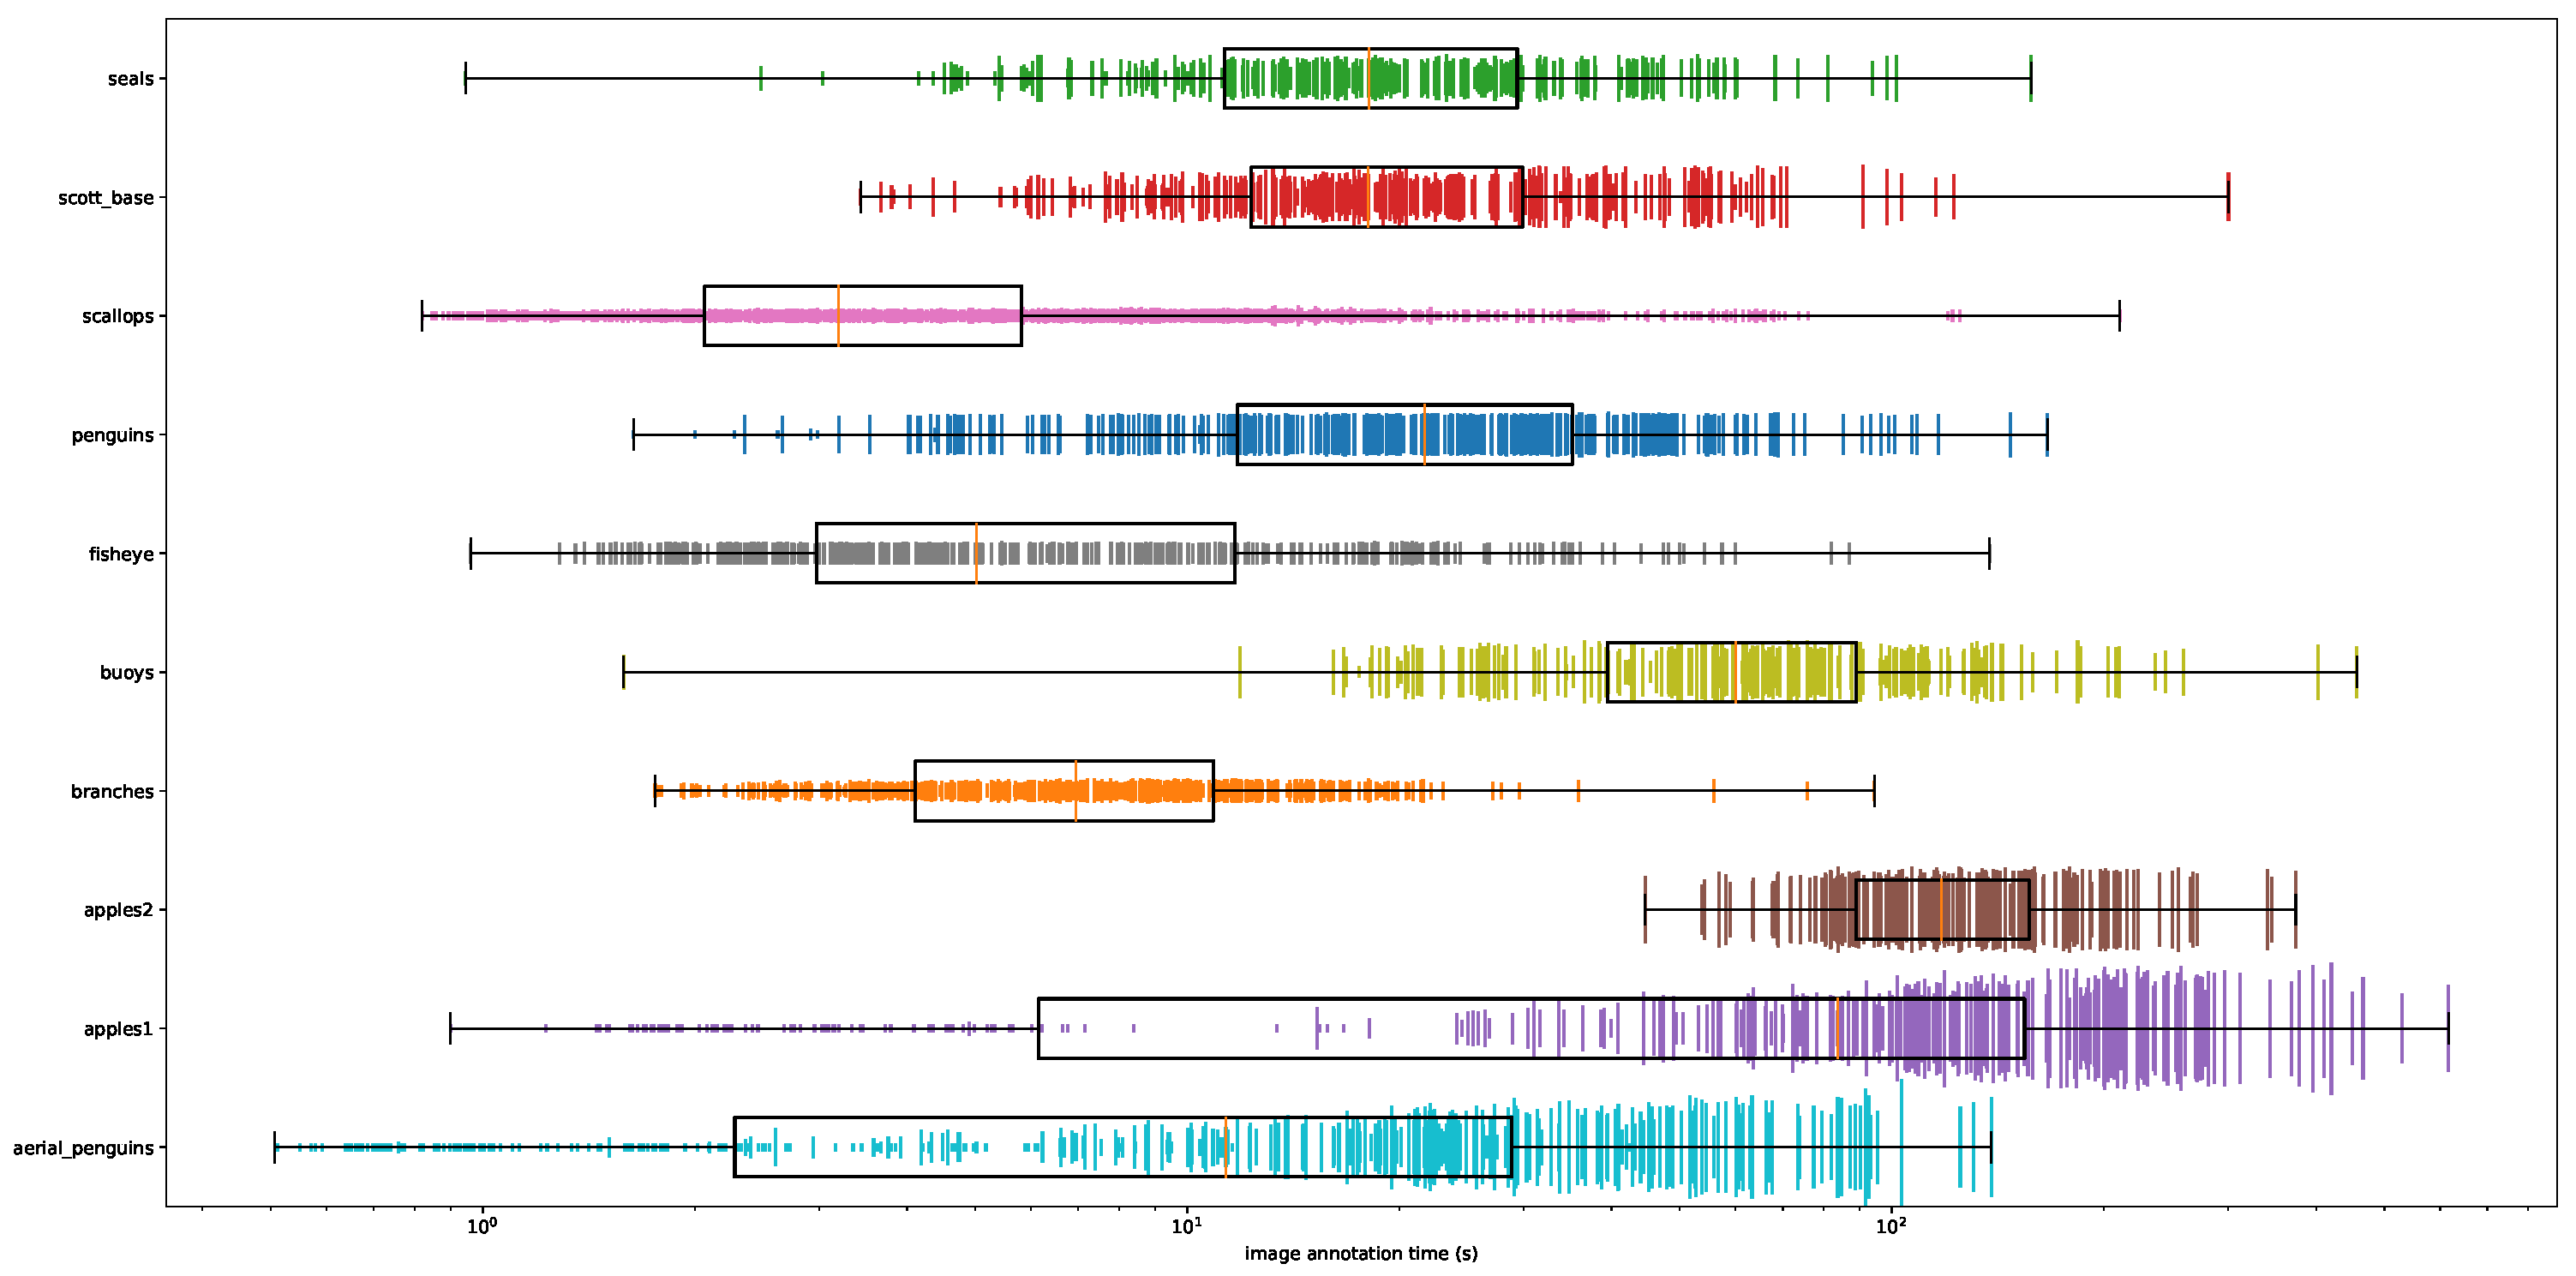
\includegraphics[width=1.0\linewidth]{charts/summaries/duration_boxplot.pdf}
\caption{ Per image annotation time distributions, vertical lines show the individual images and the height of each line is proportional to the square root of number of instances }
\label{fig:duration_boxplot}
\end{figure}




\subsection{Annotation rate}

\begin{figure}[H]
\centering
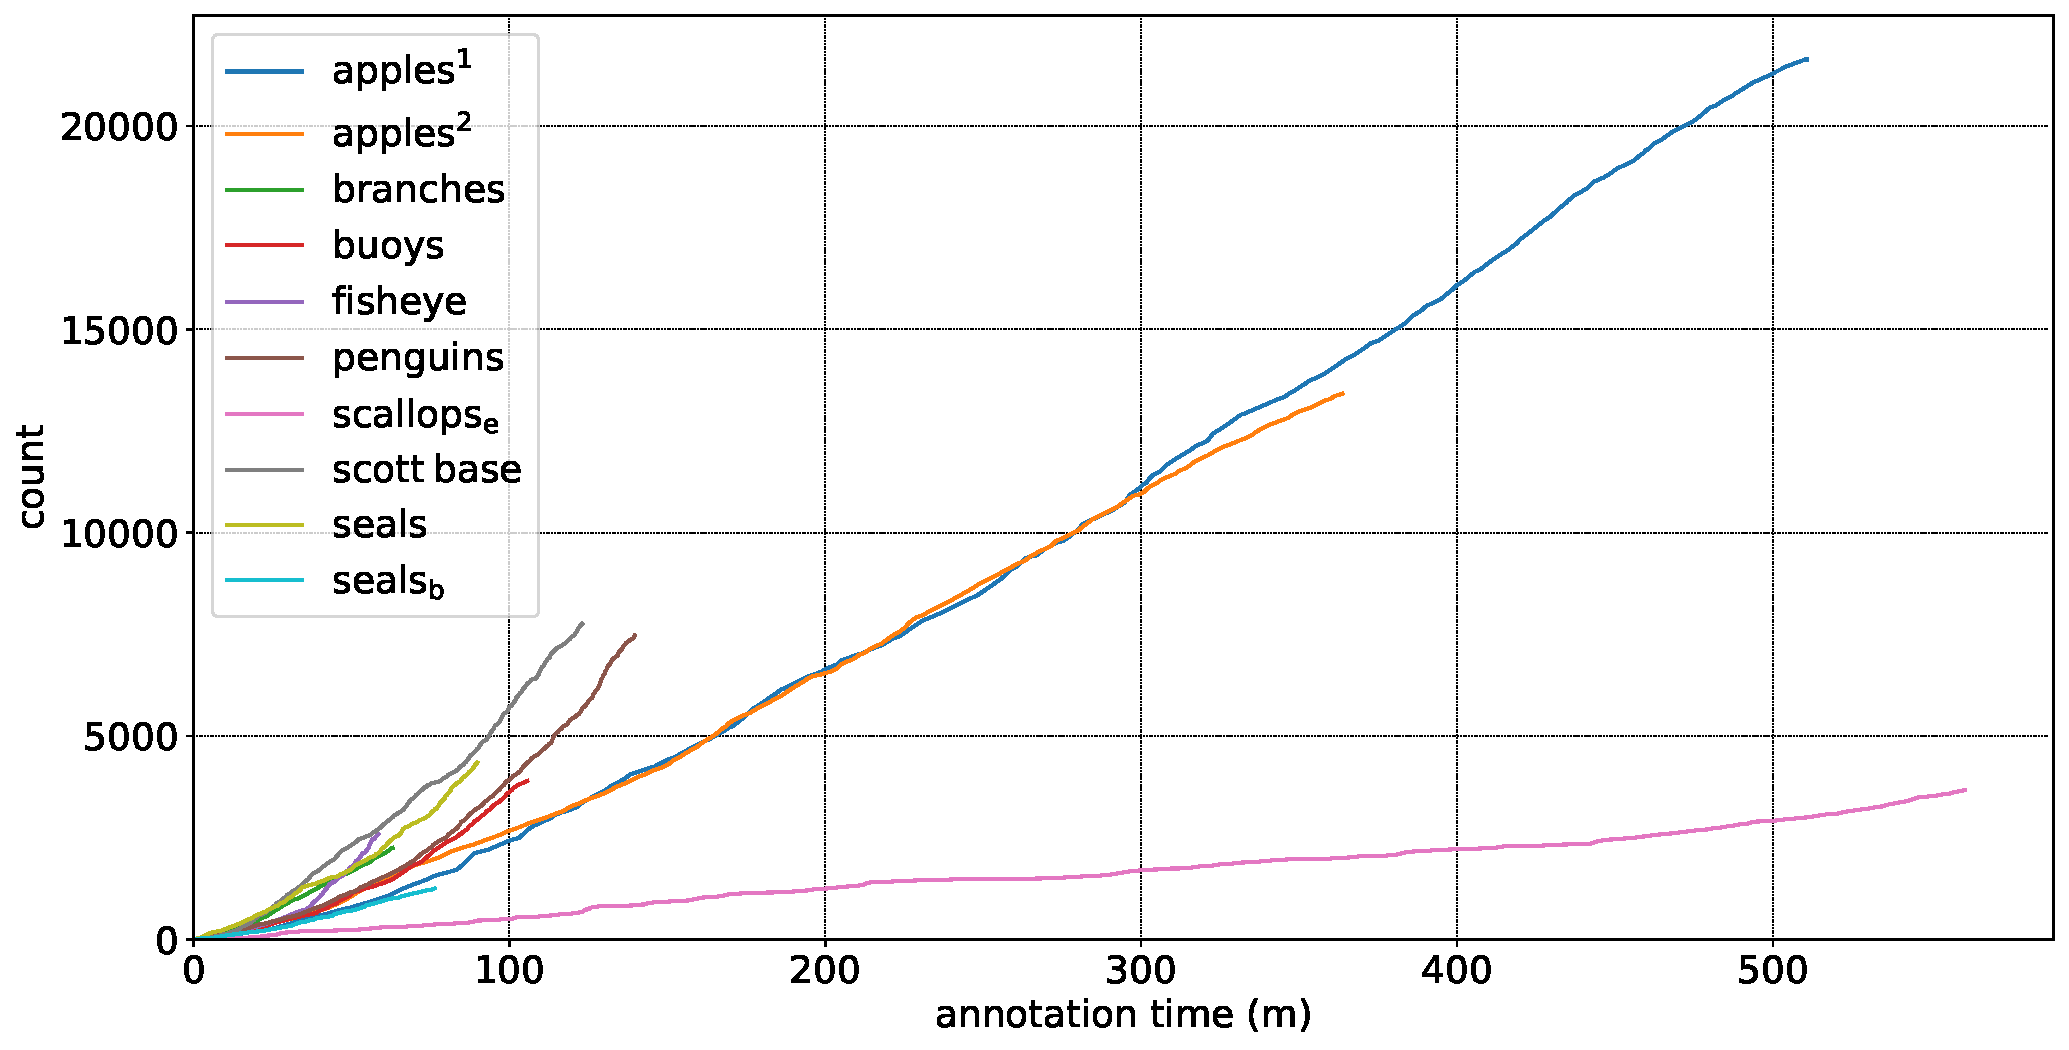
\includegraphics[width=1.0\linewidth]{charts/summaries/cumulative_instances.pdf}
\caption{ Cumulative instances annotated (truncated to first 140 minutes)  }
\label{fig:cumulative_instances}
\end{figure}



\begin{figure}[H]
\centering
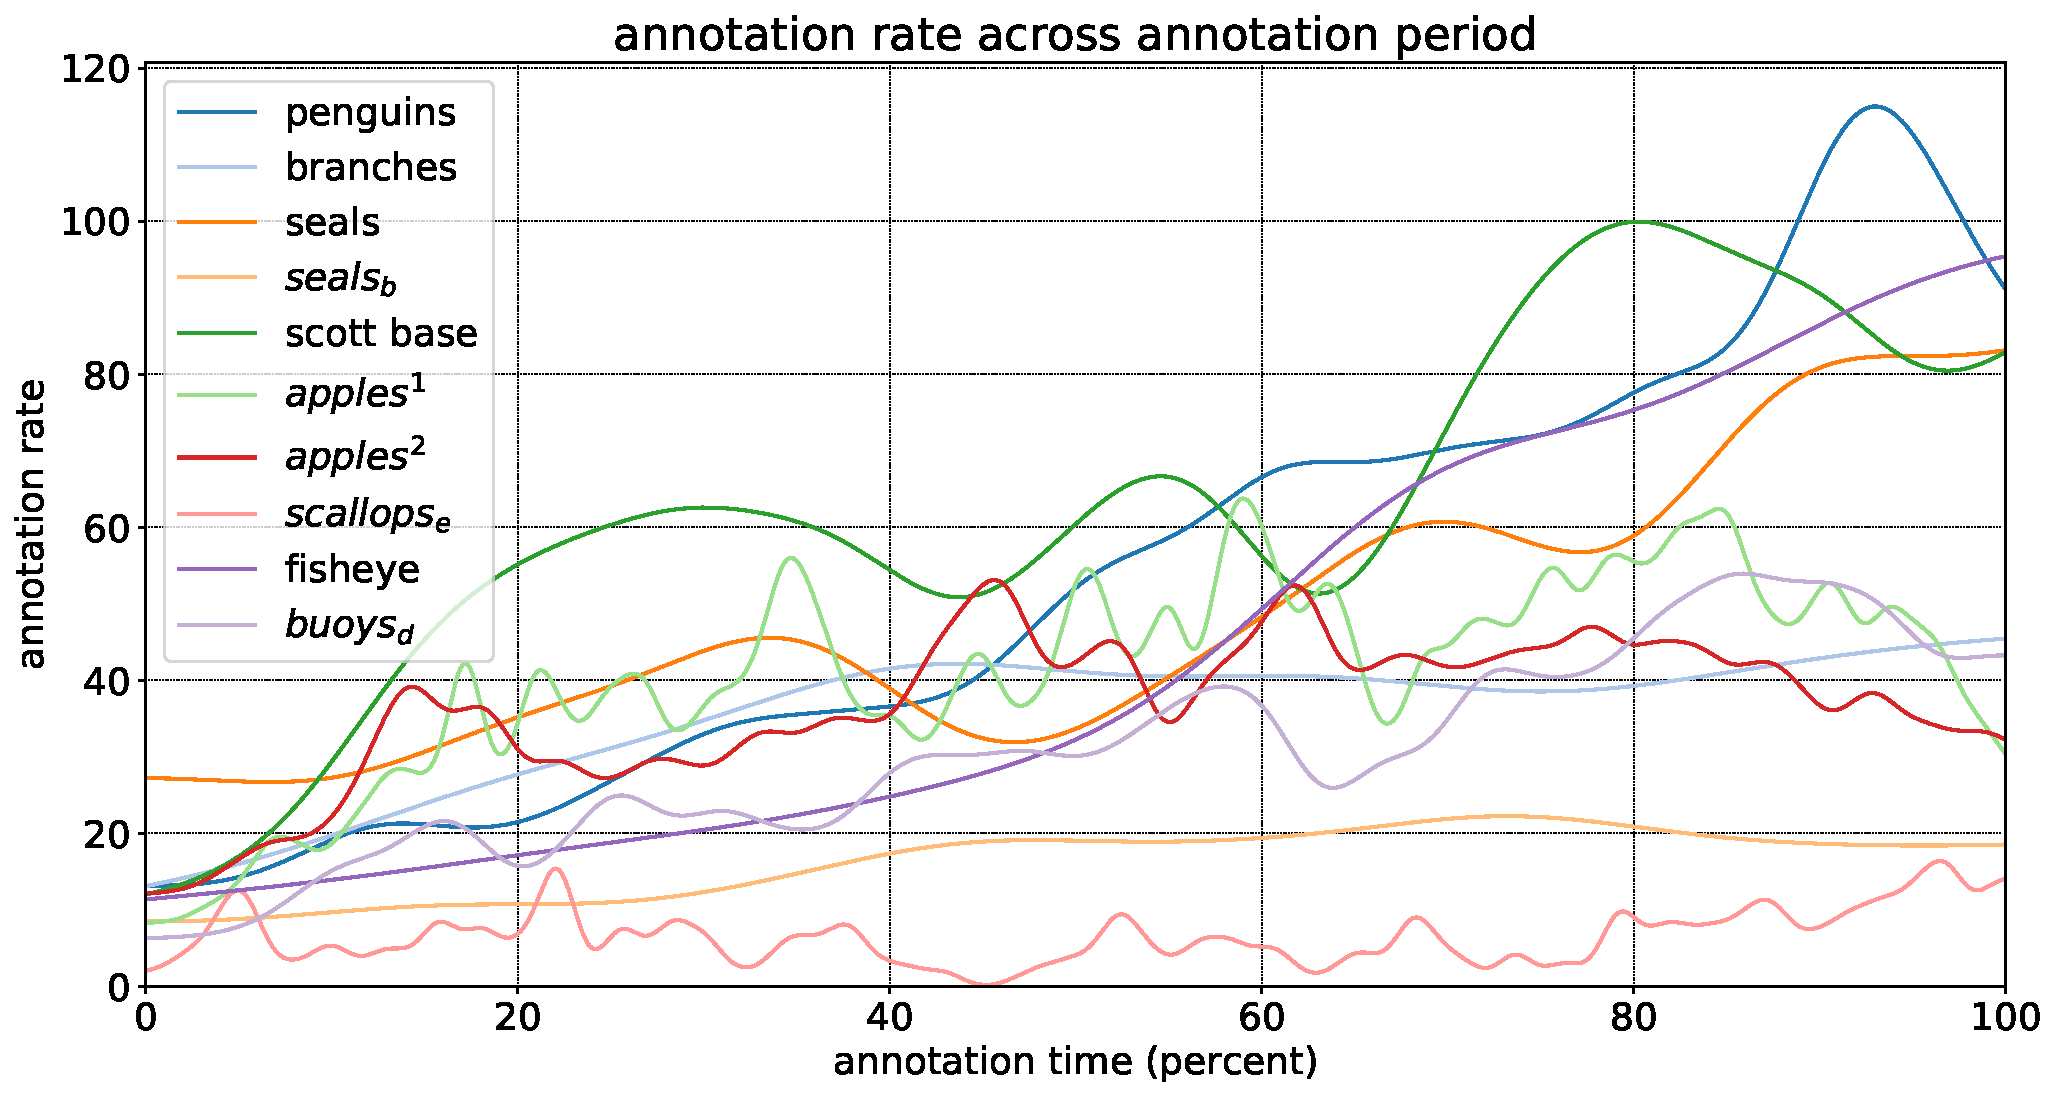
\includegraphics[width=1.0\linewidth]{charts/summaries/instance_rates.pdf}
\caption{ Annotation rate for all datasets (instances per minute) across annotation period, density plot with $\sigma=5minutes$ }
\label{fig:annotation_rate}
\end{figure}


\subsection{Continuous testing: object detection accuracy}


\begin{figure}[H]
\centering
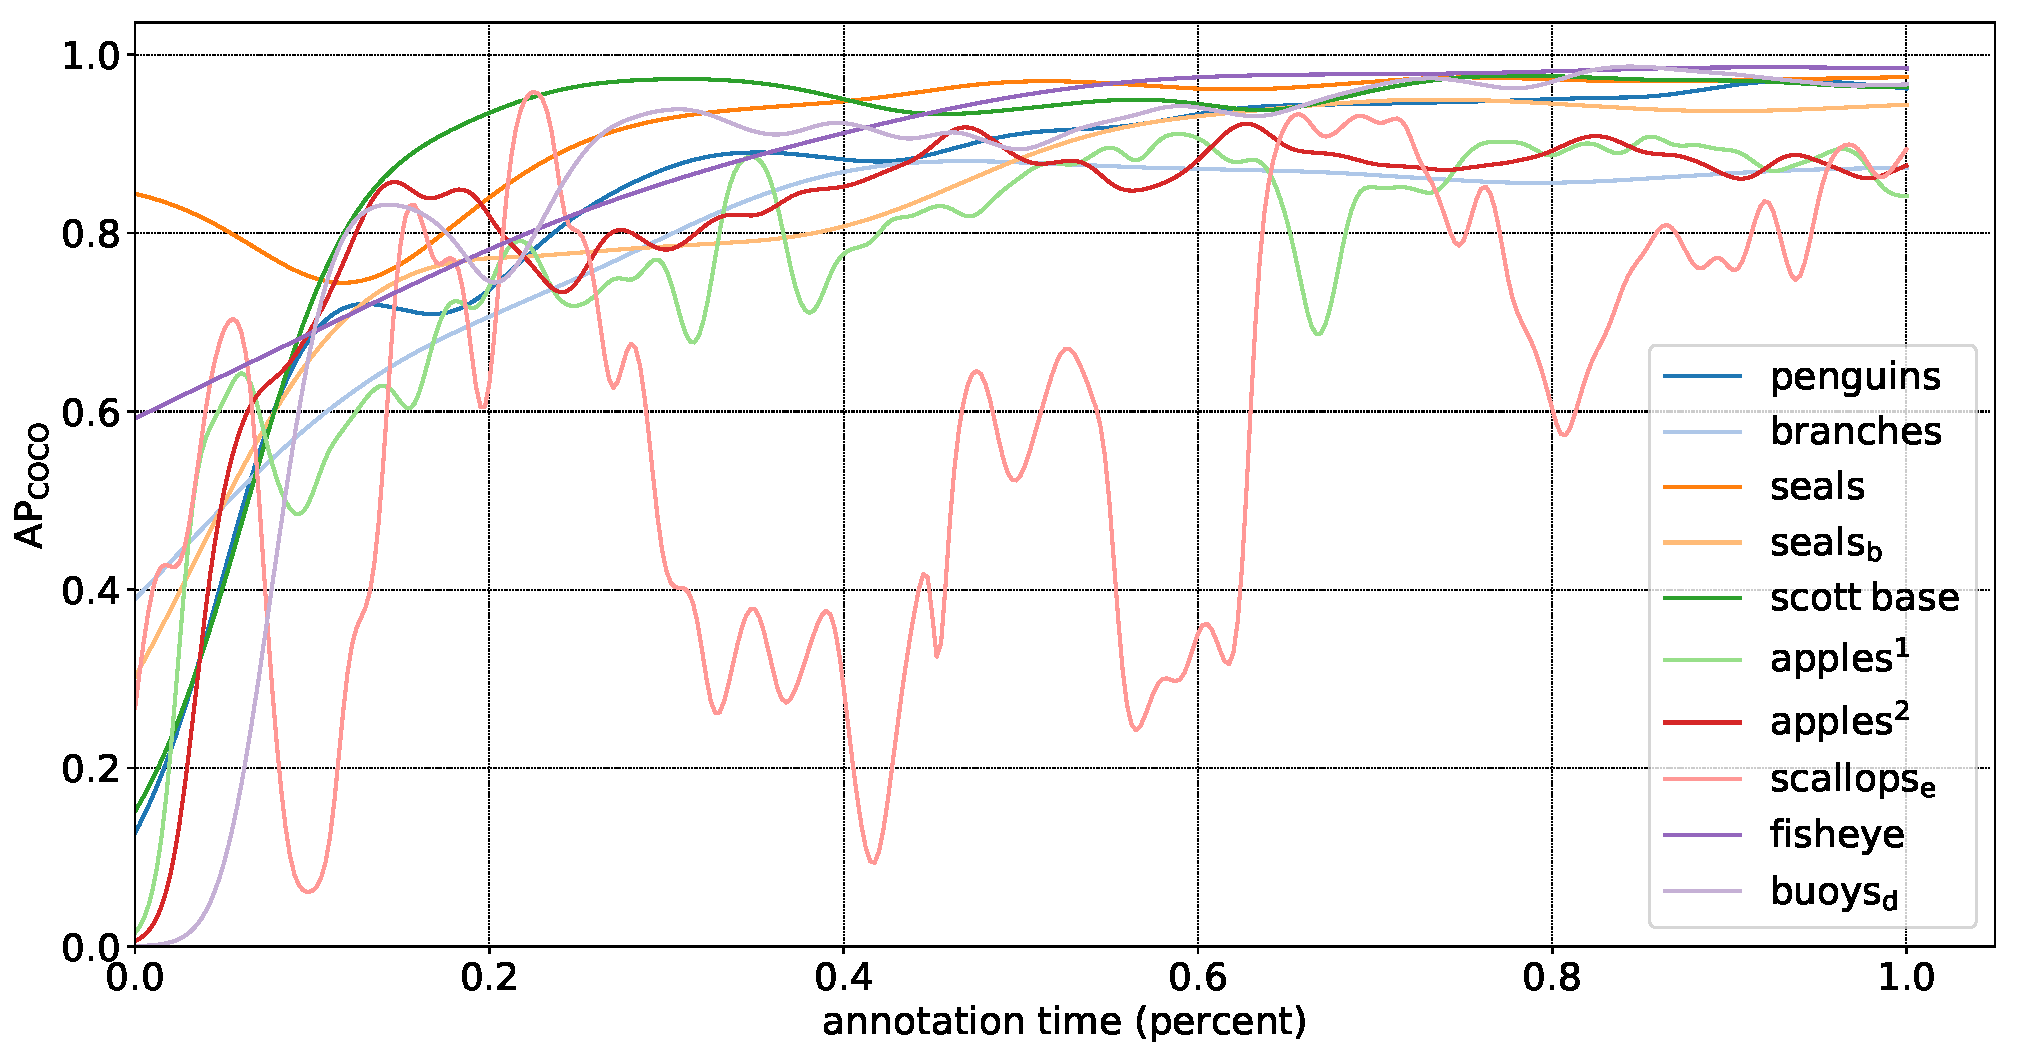
\includegraphics[width=1.0\linewidth]{charts/running_maps/overall.pdf}
\caption{ Local $AP_{COCO}$ of detections with respect to corrected annotations }
\label{fig:average_precision_test}
\end{figure}


\begin{figure}[H]
\centering
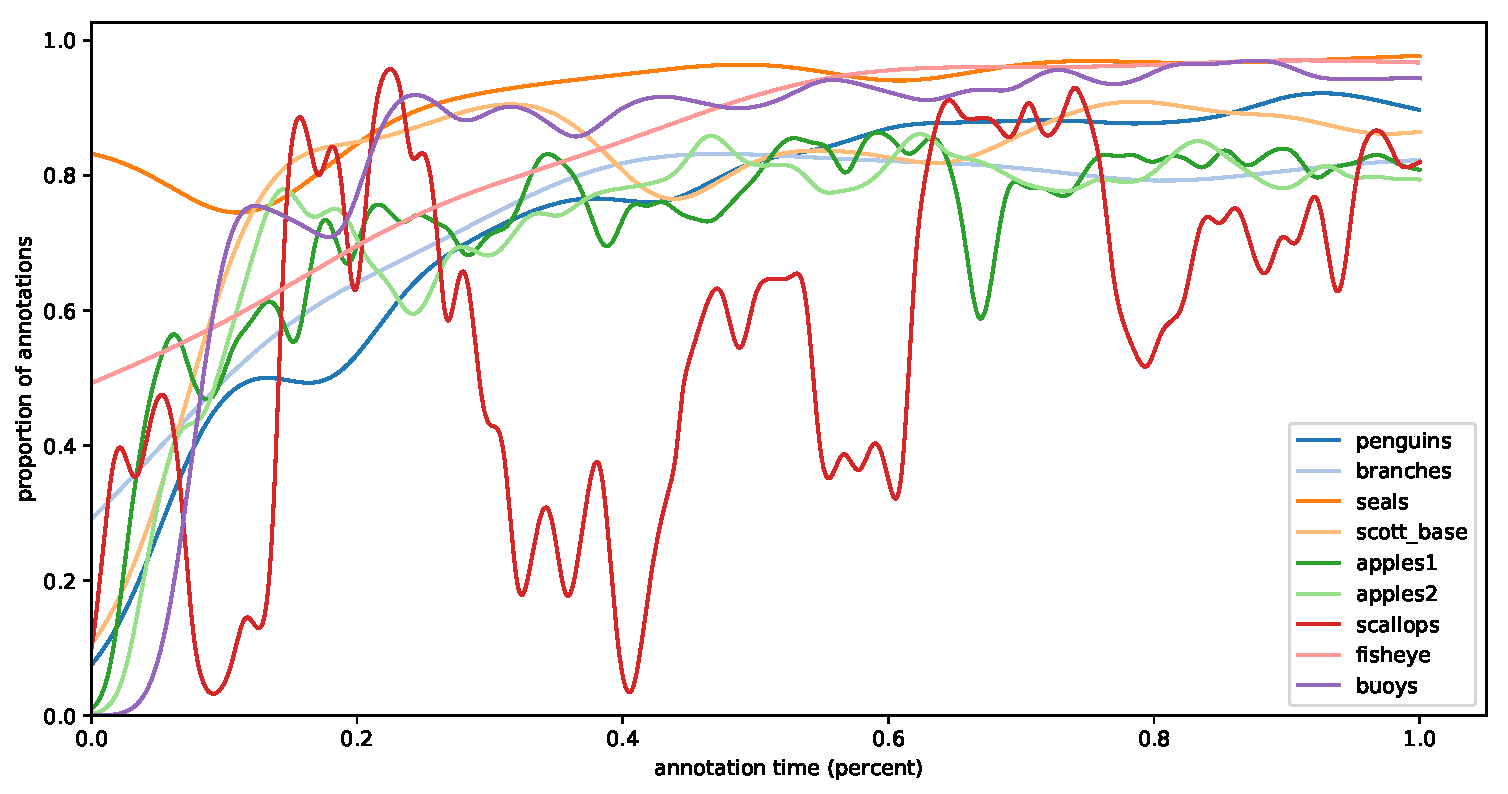
\includegraphics[width=1.0\linewidth]{charts/summaries/positive_ratio.pdf}
\caption{ Ratio of detections used unmodified as annotations after verification }
\label{fig:positive_ratio}
\end{figure}

\subsection{Localisation vs. confidence}
\label{sec:localisation_confidence}

\begin{figure}[ht]
\centering
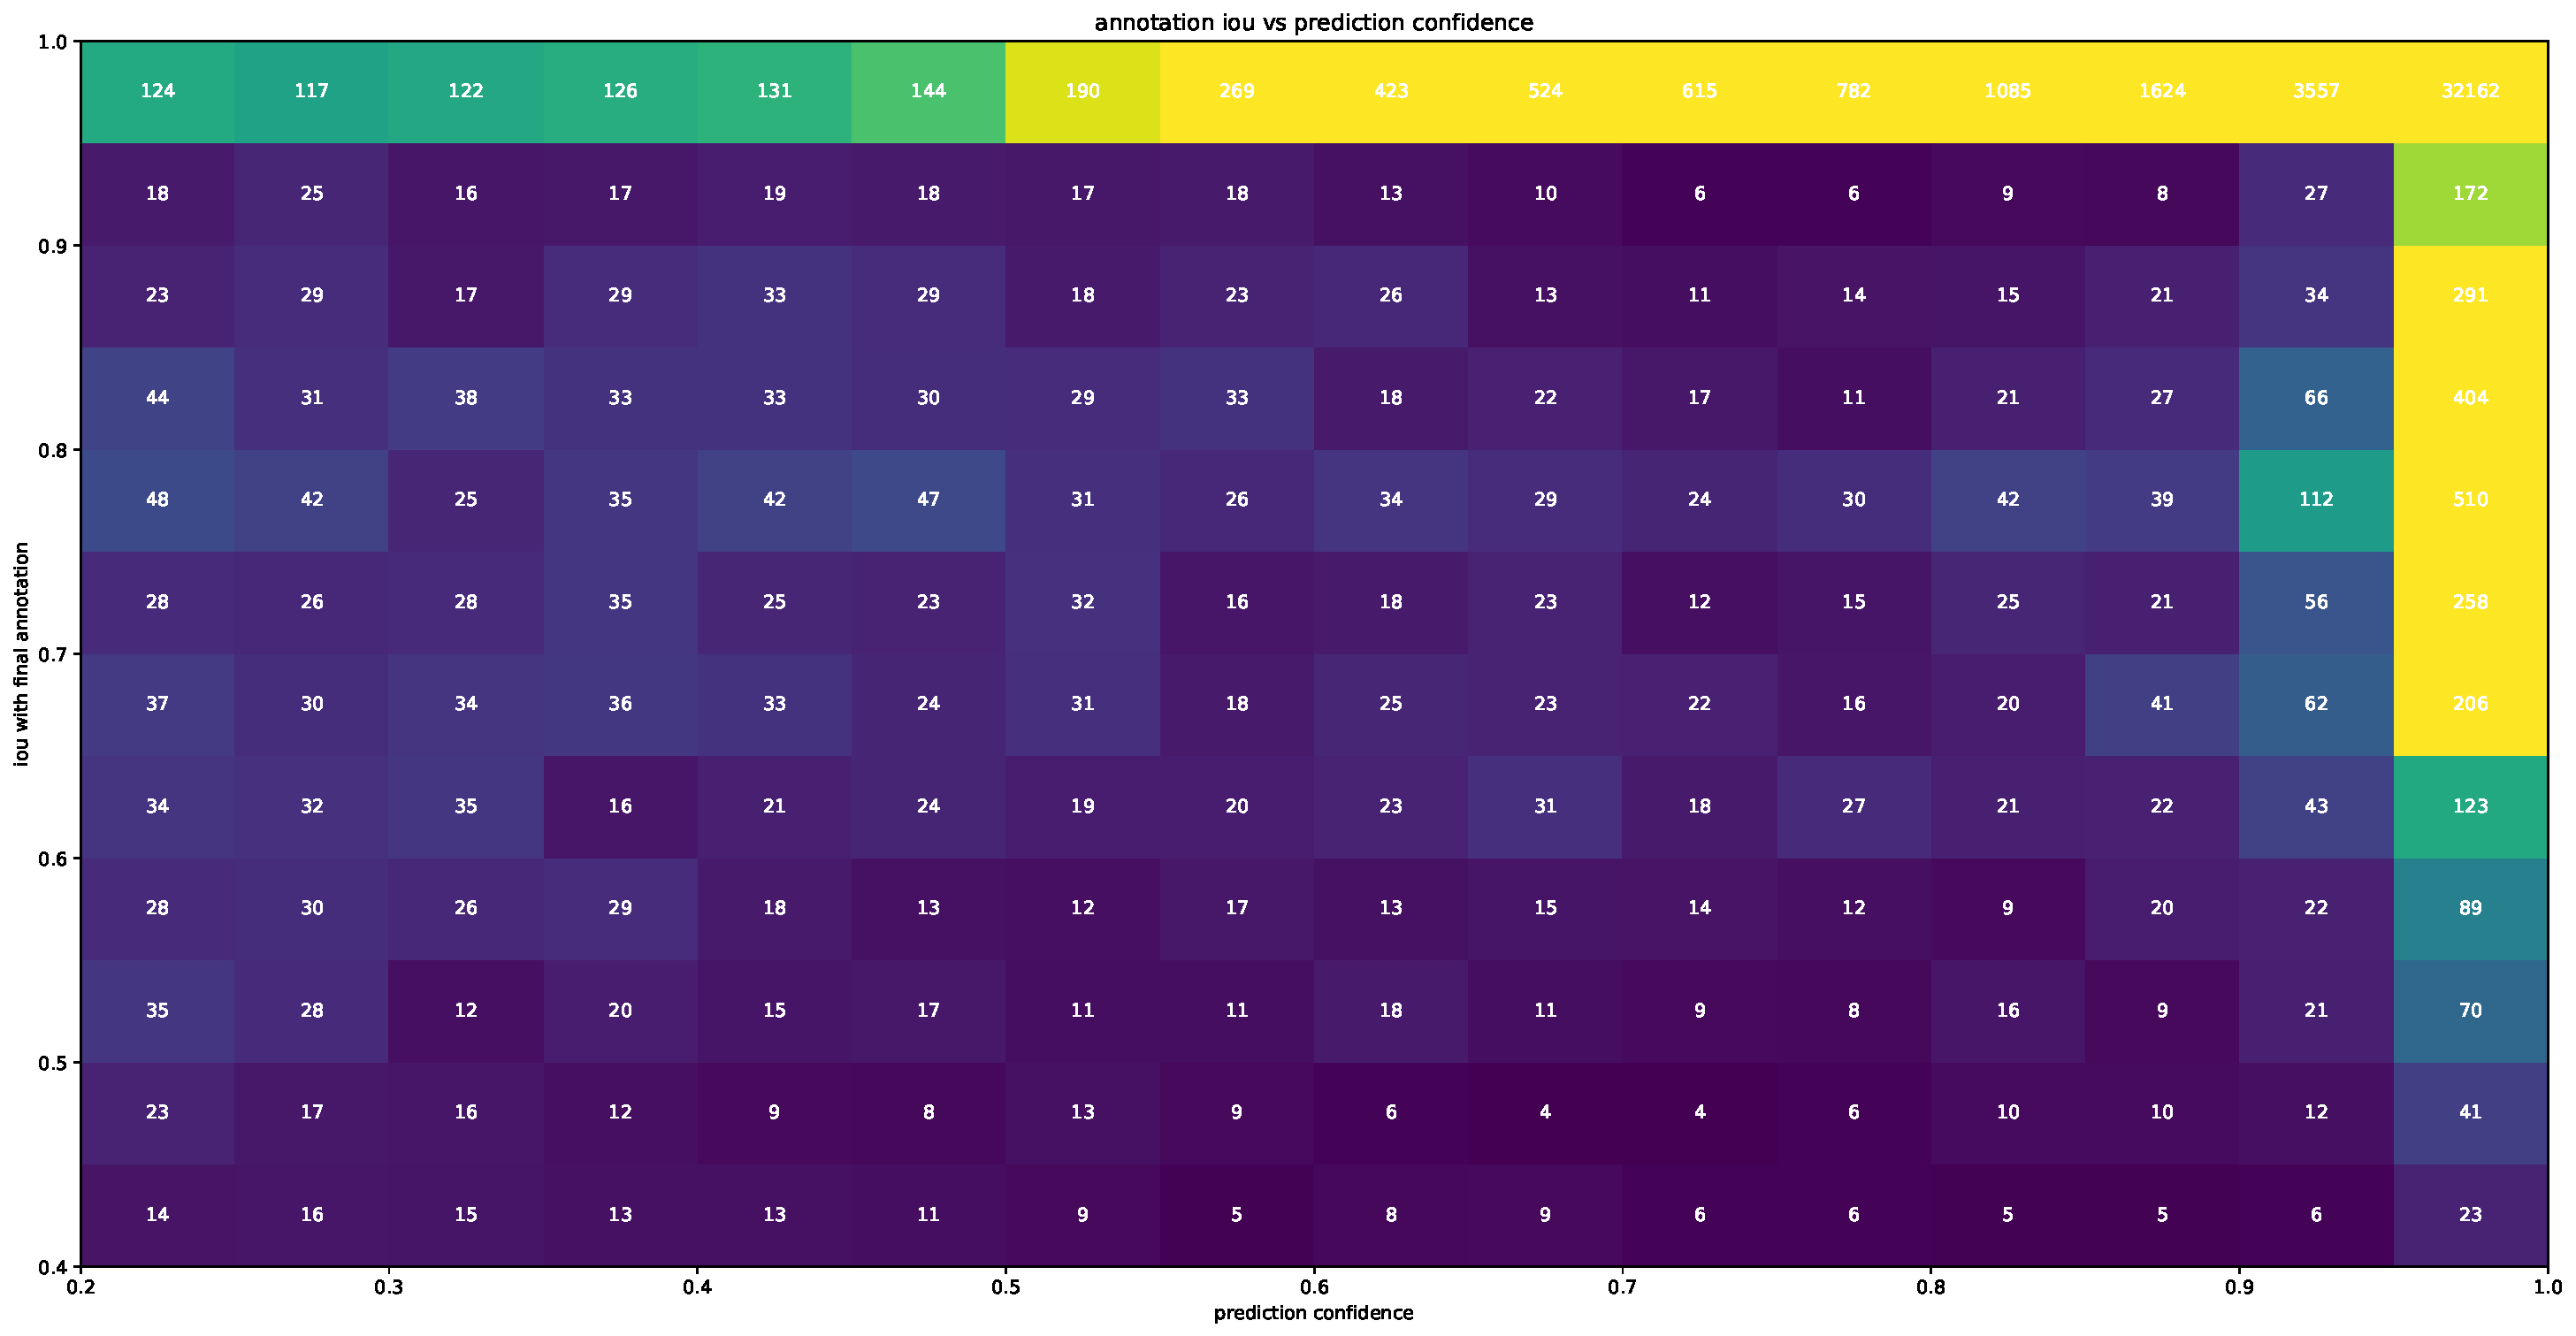
\includegraphics[width=1.0\linewidth]{charts/scatters/confidence_iou.pdf}
\caption{ IoU of detection with respect to final annotation vs. confidence, for detections (modified or otherwise) included as an annotation }
\label{fig:iou_confidence}
\end{figure}

One of the premises of providing the ability to pick and chose low confidence detections is that weakly detected objects are often be localised well. 

Figure~\ref{fig:iou_confidence} shows that is the case, both a significant proportion final annotations had low confidence, good localisation of low confidence detections are high 

\begin{table}[h]
\caption{Breakdown by dataset of detections included as an annotation; confident if $ p > 0.7 $, precise if $ IoU > 0.85 $ with respect to final annotation} 
\noindent\resizebox{1.0\textwidth}{!}{%    
\begin{tabular}{l l l l l l l l || l}
& seals  & $seals_b$ & $apples^1$ & $apples^2$ & penguins & fisheye & branches & total  \\
\toprule
high confidence, imprecise & 1.2\%  & 0.4\%     & 5.1\%      & 7.9\%      & 7.5\%    & 1.4\%   & 5.3\%    & 5.5\%  \\
low confidence, precise & 7.2\%  & 6.3\%     & 6.5\%      & 5.5\%      & 1.2\%    & 5.6\%   & 7.5\%    & 5.5\%  \\
high confidence, precise   & 90.2\% & 93.1\%    & 81.5\%     & 80.0\%     & 89.7\%   & 89.9\%  & 79.6\%   & 83.7\% \\
\bottomrule
\end{tabular}
}
\end{table}

In the implementation of object detection neural networks such as the one used in this work (see chapter~\ref{chap:object_detection}) the sub-network for classification is separate from localisation




\subsection{ Localisation precision }
\label{sec:localisation_precision}

\begin{figure}[ht]
\centering
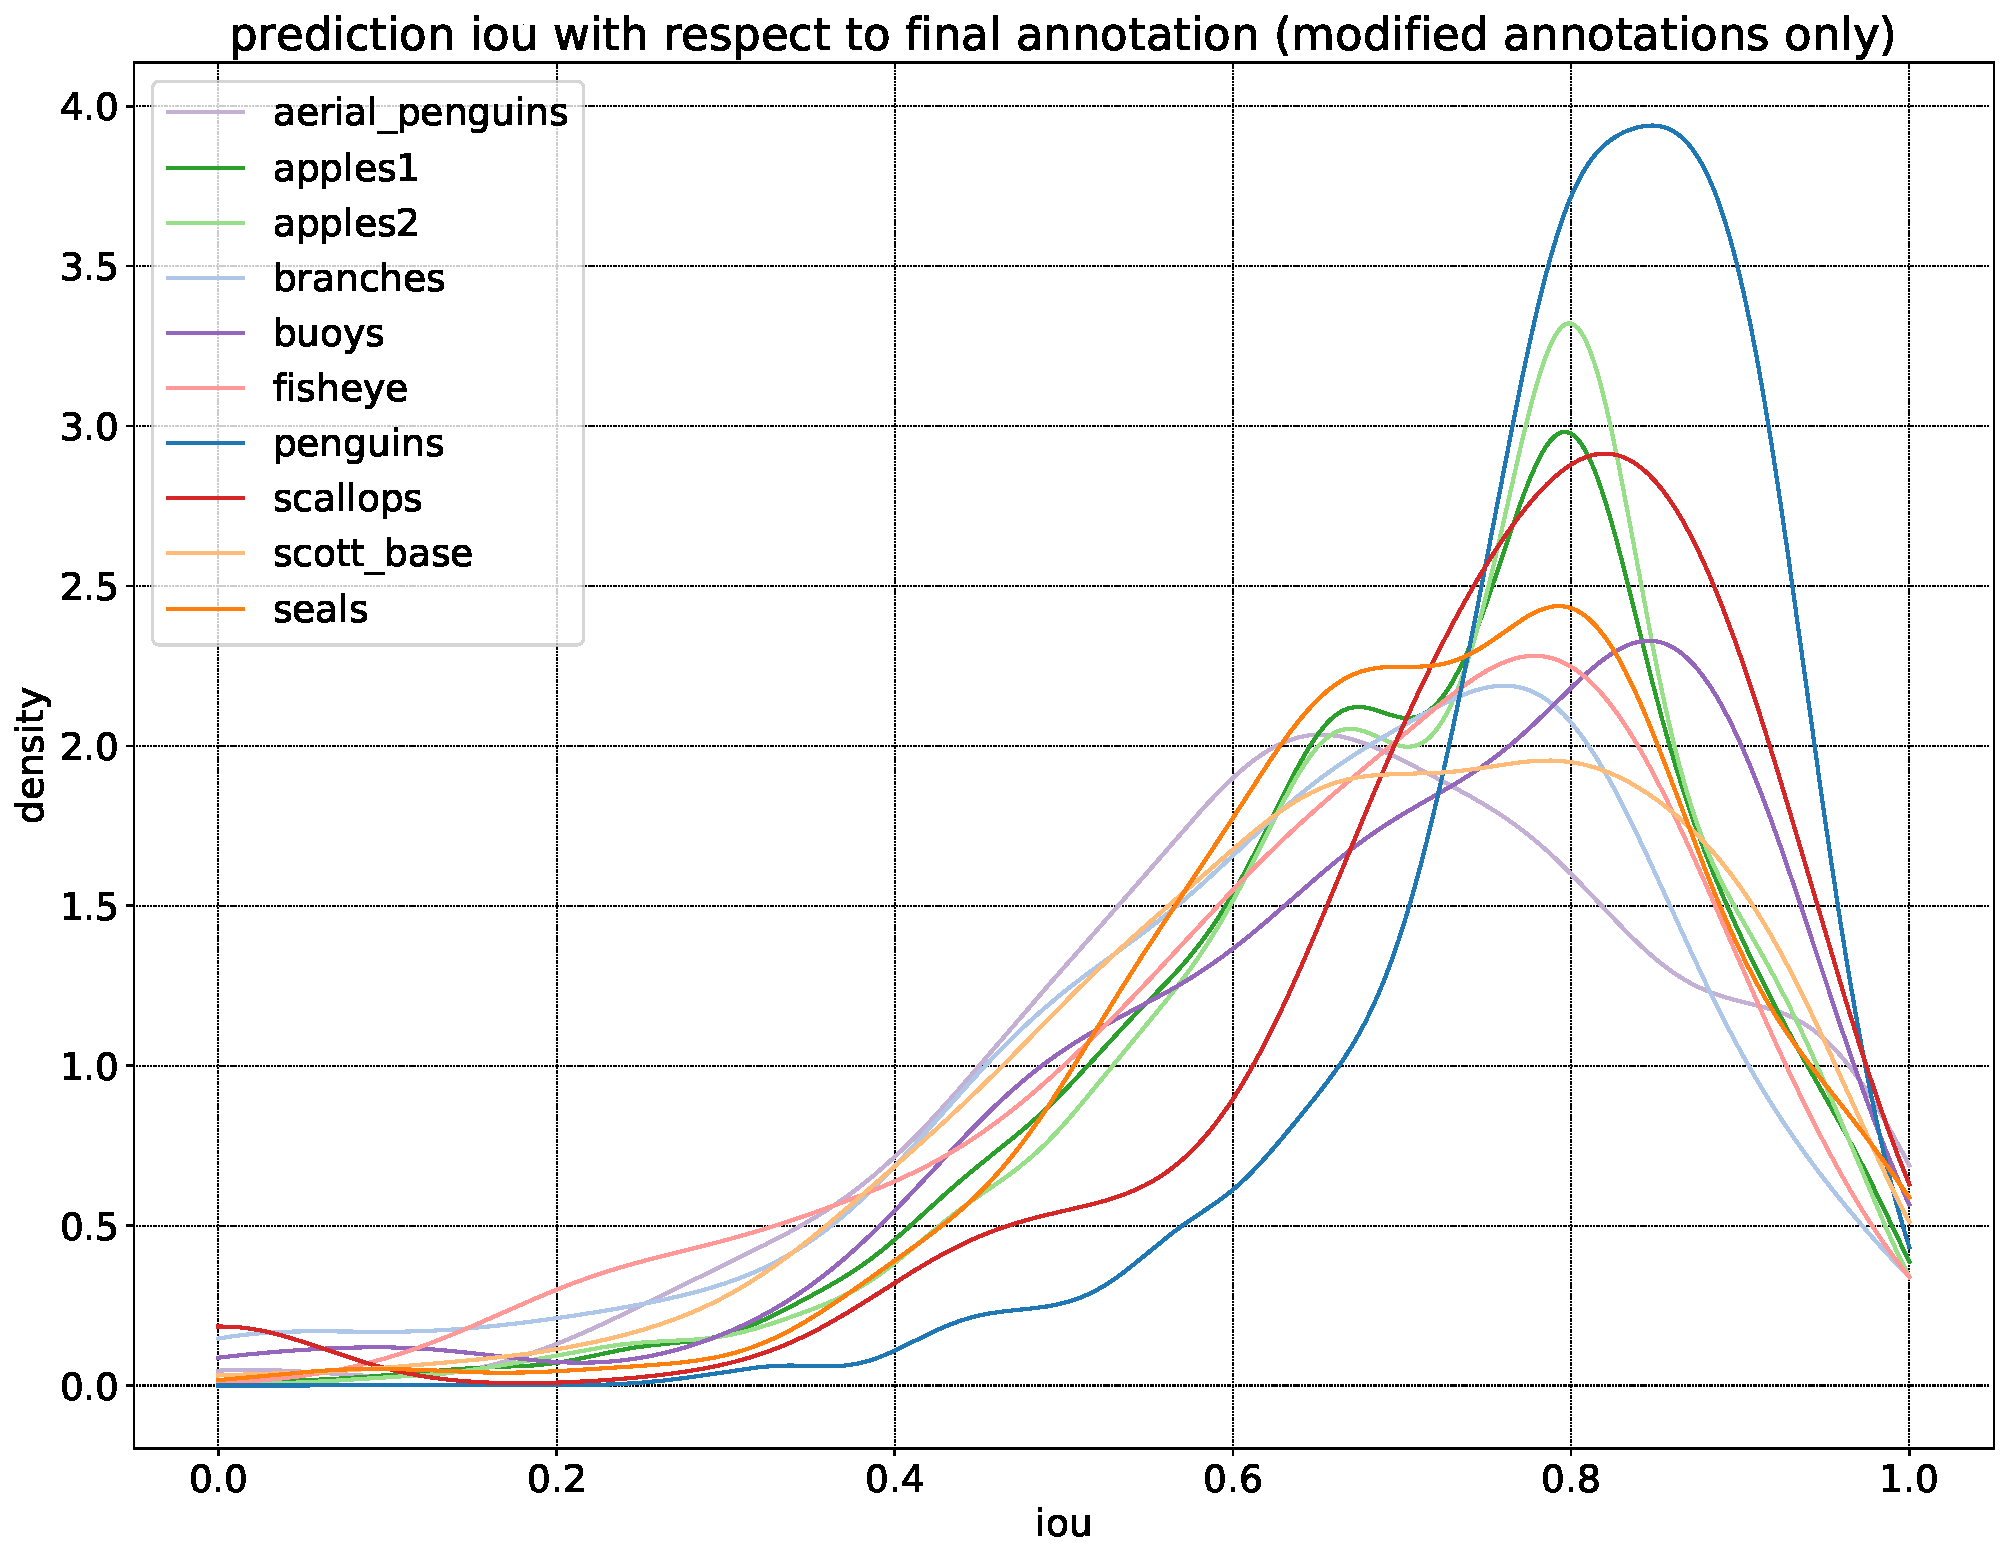
\includegraphics[width=1.0\linewidth]{charts/scatters/iou_dataset.pdf}
\caption{ Density plot of IoU for transformed annotations for each dataset }
\label{fig:density_iou}
\end{figure}



In order to verify any annotation (regardless if it was created by human annotation or machine detection), there exists an implicit localisation threshold. This threshold and the amount of variability can't be measured directly without an absolute ground truth, or by repeated annotation of the same images. It is possible however to analyse the magnitude of the corrections applied.



Human annotation has a certain amount of variability, from person to person and even annotations from the same person. For a large annotation effort a plan for annotation and quality controls can improve consistency







\section{Case study: counting Adélie penguins from aerial photographs}



One potentially useful for verification based annotation is counting things, it provides some of the time savings of automatic inference but also the accuracy of human annotation because the machine predictions are verified, and can begin without possessing an existing dataset or developing specific recognition methods.


One of the sources of inspiration for this work in verification based annotation came from \cite{McNeill2011}, where a tool was created to semi-automatically count Adelie penguins from aerial photographs. The penguins are first automatically detected, then follows a verification process allowing a human annotator to mark false positives and false negatives.

The method for detecting penguins is to first detect penguin colonies which can be done many times by the unique colour of the penguin guano. Individual penguins were then identified by thresholding and local minima detection and culling of long thin objects. 

The images (two of which can be seen in figure~\ref{fig:penguin_examples}), originate from aerial photographic surveys \cite{Lyver2014}, from high resolution photographs, taken from 2000-2500 feet. In the case of the two images from Cape Cotter and Hallet in figure~\ref{fig:penguin_examples}, the images are cropped from images of size $ 6720\times4480 $. The Cape Royds images are spliced together from three images with various areas masked out, this was done by filling in the overlapping and irrelevant areas using a paint program.

The study which has been conducted from 1981 until present, prior to 2010 involved manually counting individual penguins using a pin to manually mark penguins and avoid duplication. 





\begin{figure*}[h!]
\centering
\begin{subfigure}[t]{1.0\linewidth}
  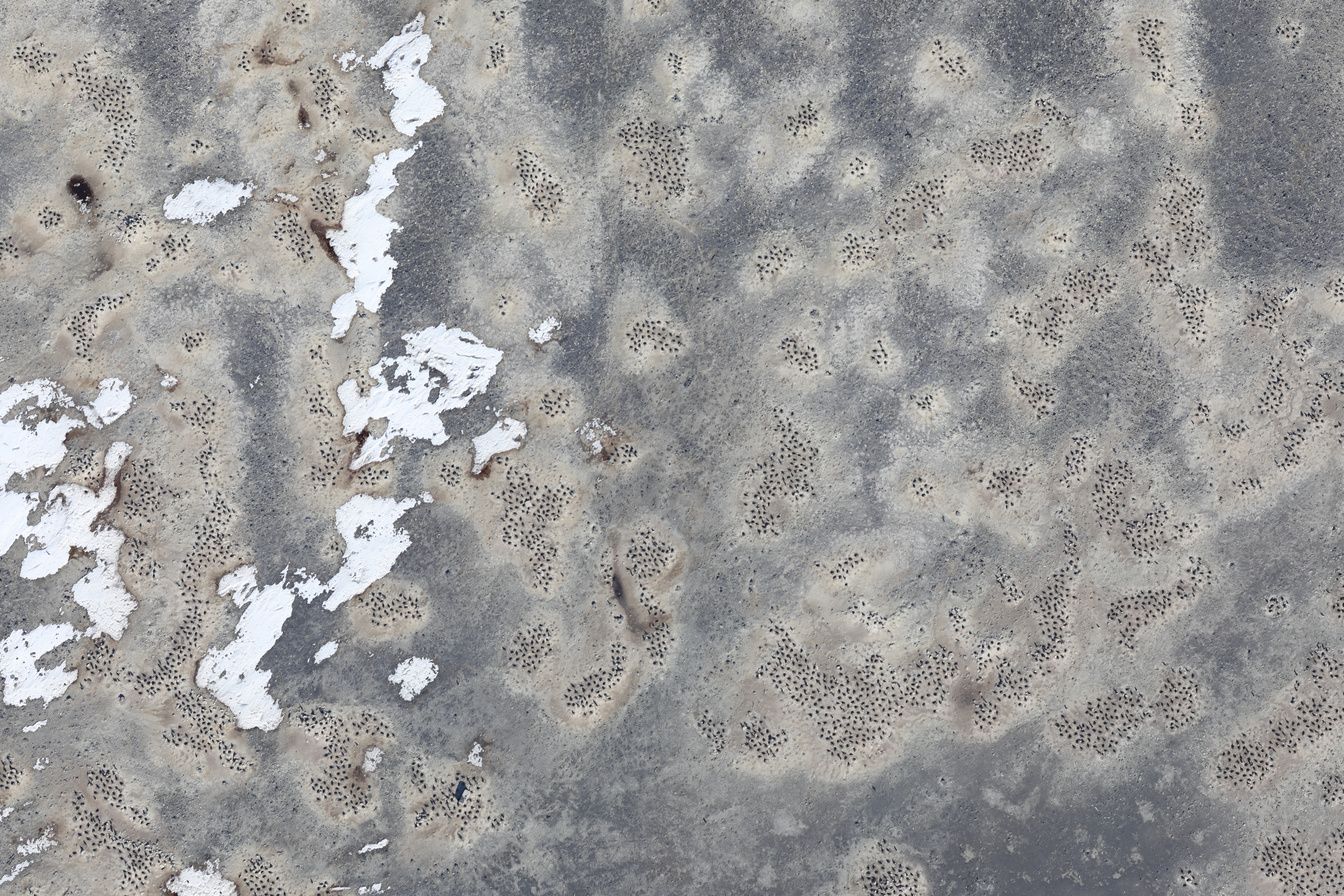
\includegraphics[width=0.475\linewidth]{figures/annotation/penguin/hallet_large.jpg}
  \hfill
  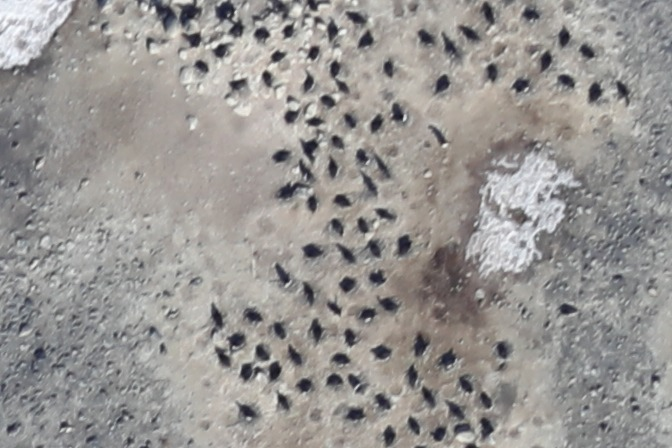
\includegraphics[width=0.475\linewidth]{figures/annotation/penguin/hallet.jpg}
  \caption{Cape Hallett 2017}
\end{subfigure}
\begin{subfigure}[t]{1.0\linewidth}
  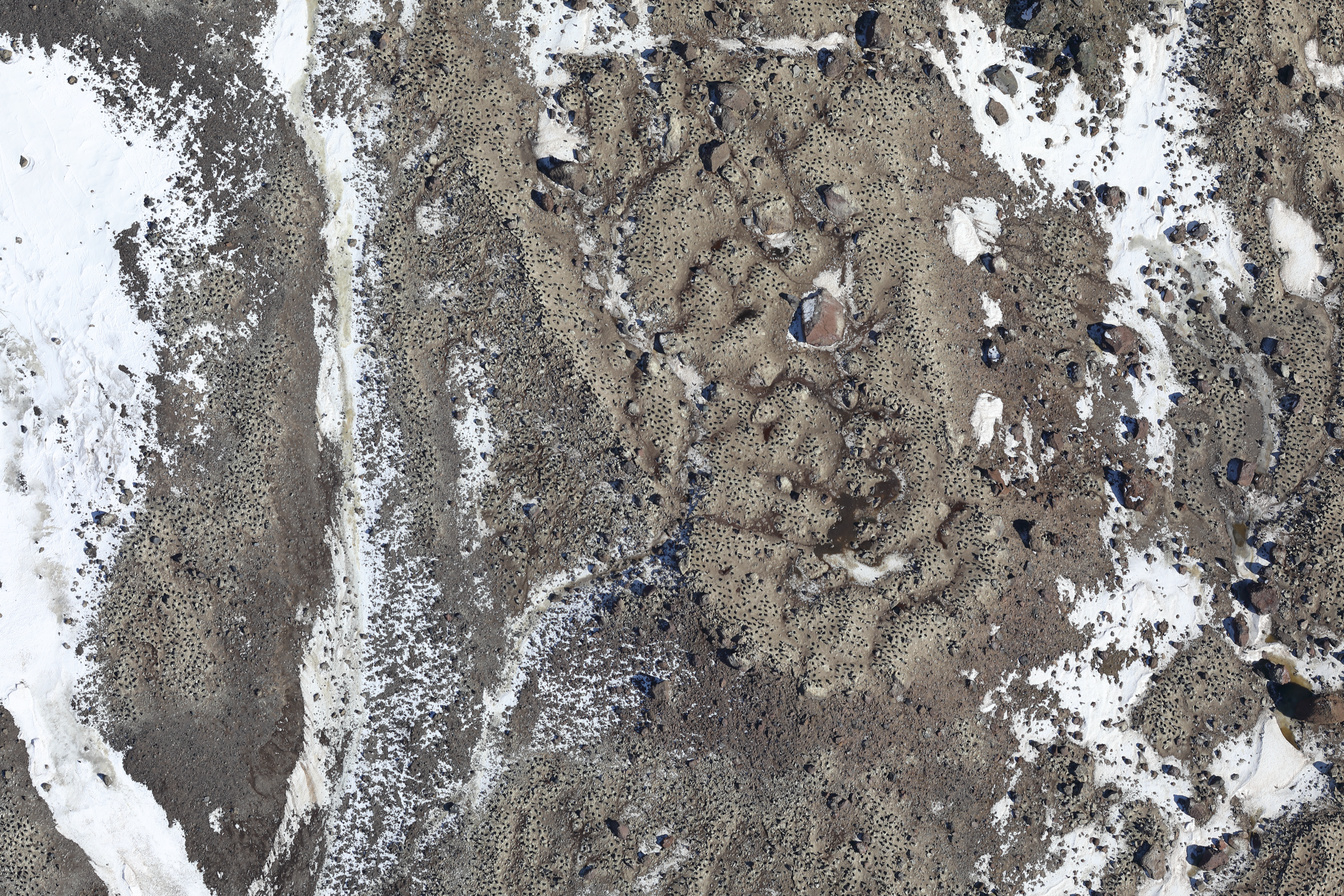
\includegraphics[width=0.475\linewidth]{figures/annotation/penguin/cotter_large.jpg}
  \hfill 
  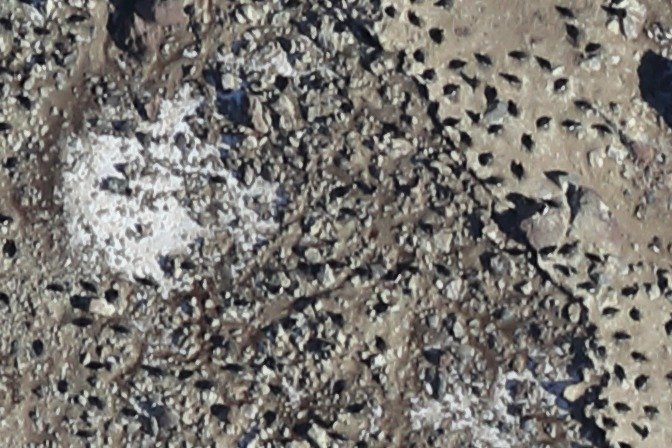
\includegraphics[width=0.475\linewidth]{figures/annotation/penguin/cotter.jpg}
  \caption{Cape Cotter 2017}
\end{subfigure}
\begin{subfigure}[t]{1.0\linewidth}
  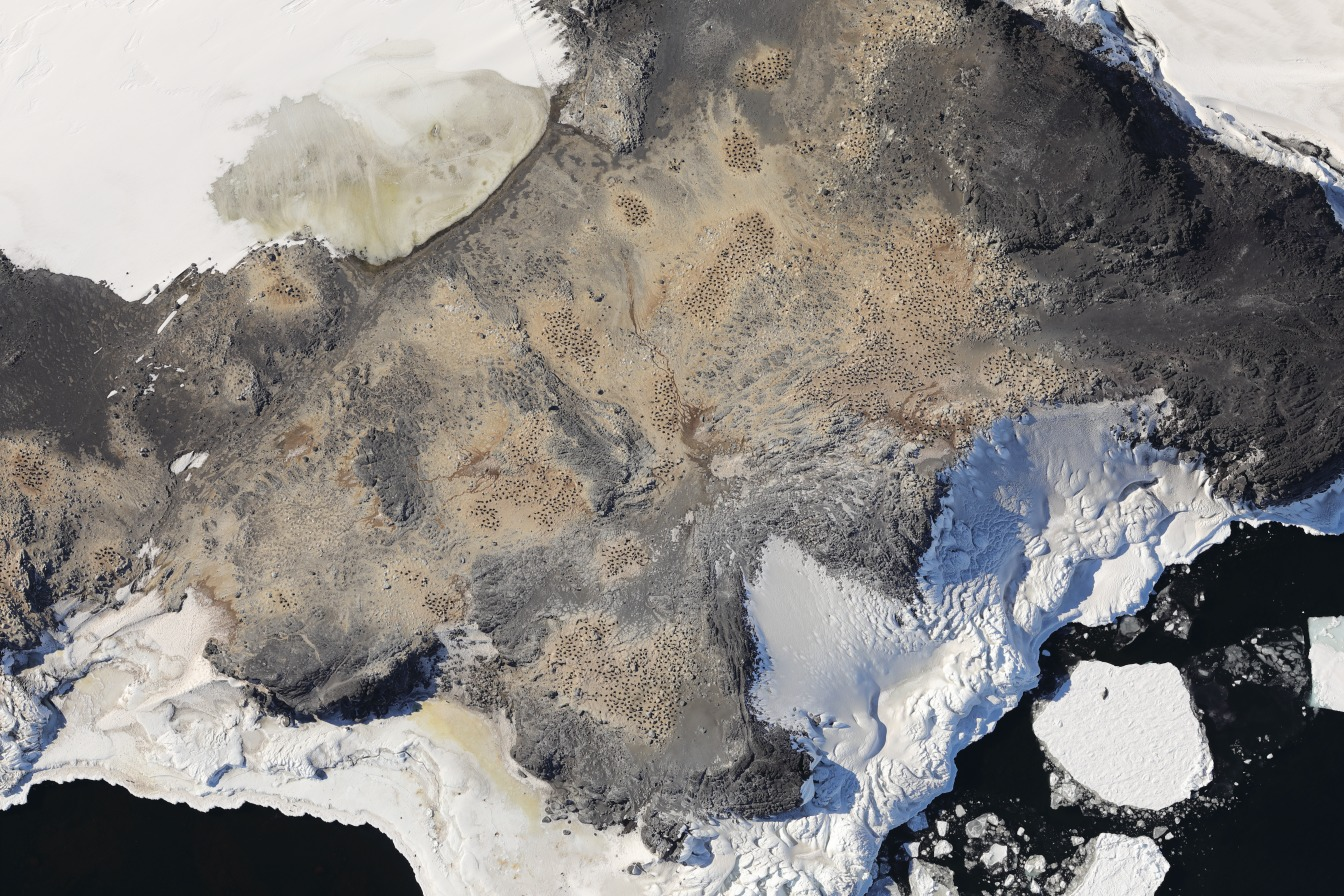
\includegraphics[width=0.475\linewidth]{figures/annotation/penguin/royds_large.jpg}
  \hfill
  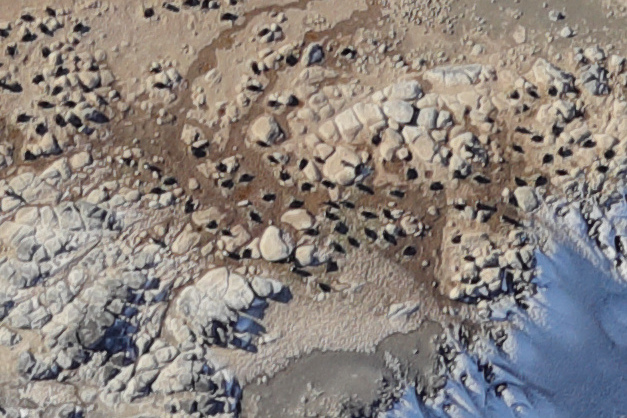
\includegraphics[width=0.475\linewidth]{figures/annotation/penguin/royds.jpg}
  \caption{Cape Royds 2017}
\end{subfigure}

\caption{Examples from the Adelie penguin census data taken in 2017. On the left hand column are images showing the zoomed out landscape, on the right are representative crops zoomed in.  In (a) an image from Cape Hallet image showing clearly visible, easy to identify penguins as dark patches. In (b) Cape Cotter showing many more difficult to identify penguins, often with a high degree of ambiguity not only for the machine learning algorithm but for a human annotator, in rocky areas especially shadows from rocks are very difficult to discern from penguins. In (c) Cape Royds, a smaller colony to the other two (and complete). In terms of ambiguity and uncertainty somewhere in-between. }
\label {fig:penguin_examples}
\end{figure*}


\subsection {Effect of uncertainty}

 The strength of the object detector has an effect on the usefulness of verification. If a detector is weak and the noise of many inaccurate detections overwhelms the number of any accurate detections, verification becomes less effective - and manual annotation becomes more efficient. When the source images are very uncertain this presents a challenge not only for the object detector which may be relatively weaker as a result, but for the human annotator. Many of the penguin instances to the untrained eye appear very similar to the shadow cast by rocks and difficult to discern. The nature of the imagery from the different sites shown in figure~\ref{fig:penguin_examples} provide a test case to compare the effectiveness of verification with different levels of uncertainty in the source image. 

\subsection {Method}

Separately I annotated the three sets of penguins using the annotation tool. I used circular annotations as the precise location of the penguins is of no consequence for counting applications, and in general the penguins separate themselves with a wide berth (when viewed from above).  

The very large original images were split into images of size $ 672\times448 $ (Cape Royds images were of similar size, but not exactly the same because the source images were of different size, rather than one big image like the other two). Image crops of those image, sized $ 300\times300 $ were then used during training.

\begin{table}[ht]
  \centering
    \caption{Statistics from the thee penguin sources. }
  \begin{tabular}{ l  l  l  l  l }
    Image set & Total & Images & Validation & $AP_0.5$ \\
    \toprule
    Cape Hallett  & 4217 & 100 & 683 & 0.97 \\
    Cape Cotter   & 6180 & 100 & 973 & 0.72  \\
    Cape Royds    & 2754 & 61 & 477  & 0.88 \\
    \bottomrule
  \end{tabular}

\label{fig:penguin_statistics}
\end{table}





\subsection{Results and discussion}
 
The difference in difficulty can clearly be seen in the difference of mAP in figure~\ref{fig:penguin_statistics}, where the Cape Hallet penguins were detected with almost perfect accuracy, whereas Cape Royds was more difficult and Cape Cotter considerably more difficult. 





\subsection{Case Study: Analysing Waddell Seal Counts}



\begin{figure*}[h!]
\centering
\begin{subfigure}[t]{1.0\linewidth}
  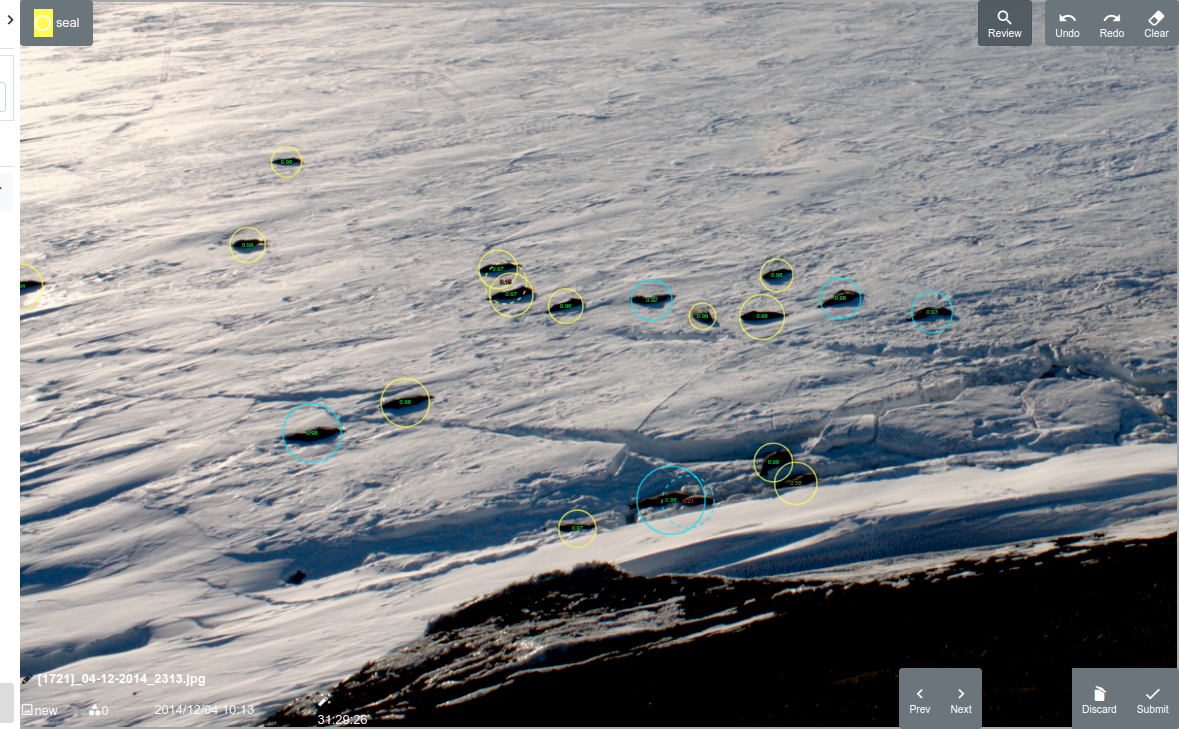
\includegraphics[width=0.475\linewidth]{figures/annotation/screenshots/seals_small2.png}
  \hfill
  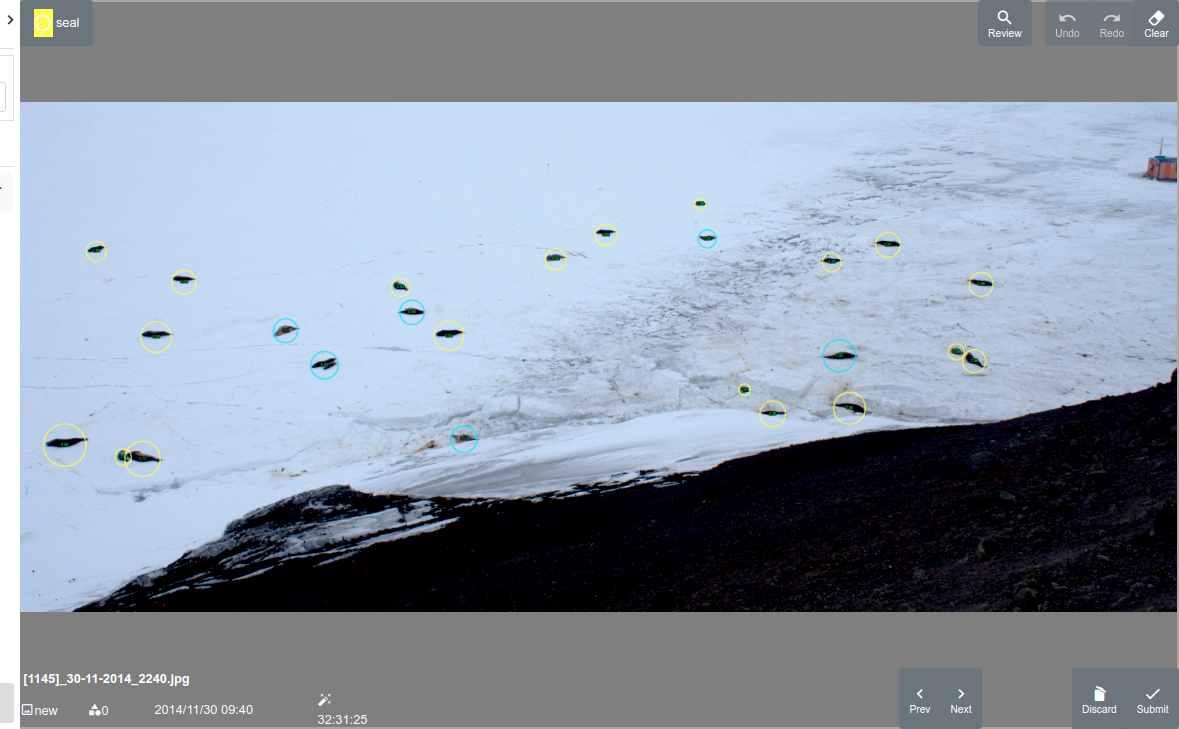
\includegraphics[width=0.475\linewidth]{figures/annotation/screenshots/seals_small.png}
  \caption{}
\end{subfigure}

\begin{subfigure}[t]{1.0\linewidth}
  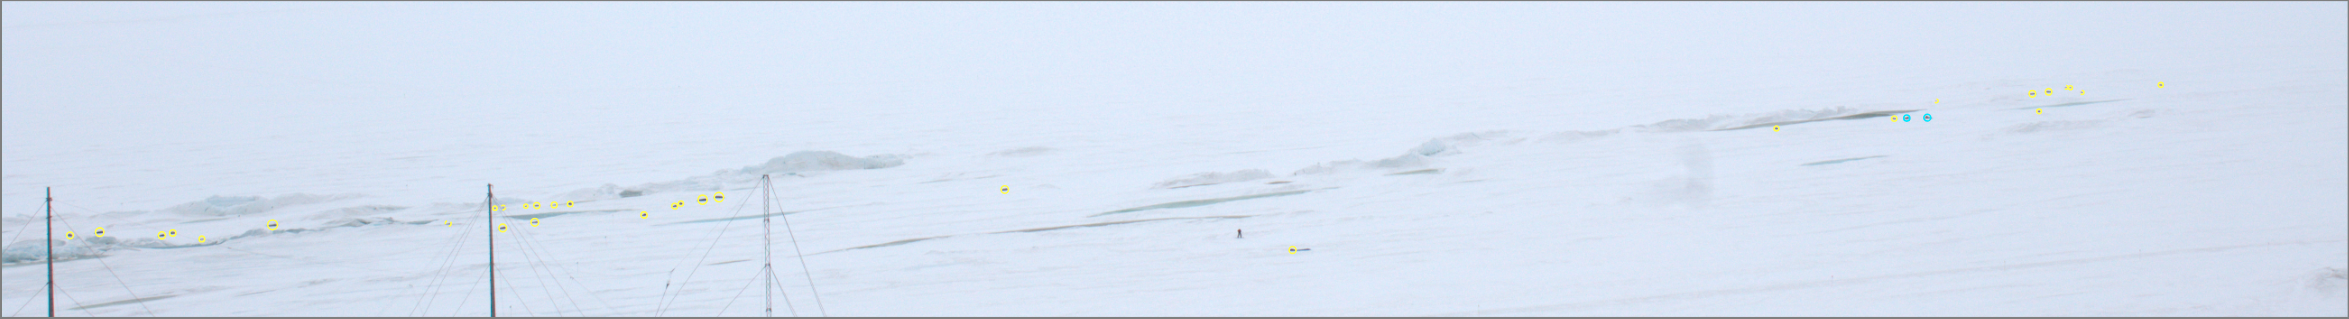
\includegraphics[width=1.0\linewidth]{figures/annotation/screenshots/cam_c.png}
\end{subfigure}

\begin{subfigure}[t]{1.0\linewidth}
  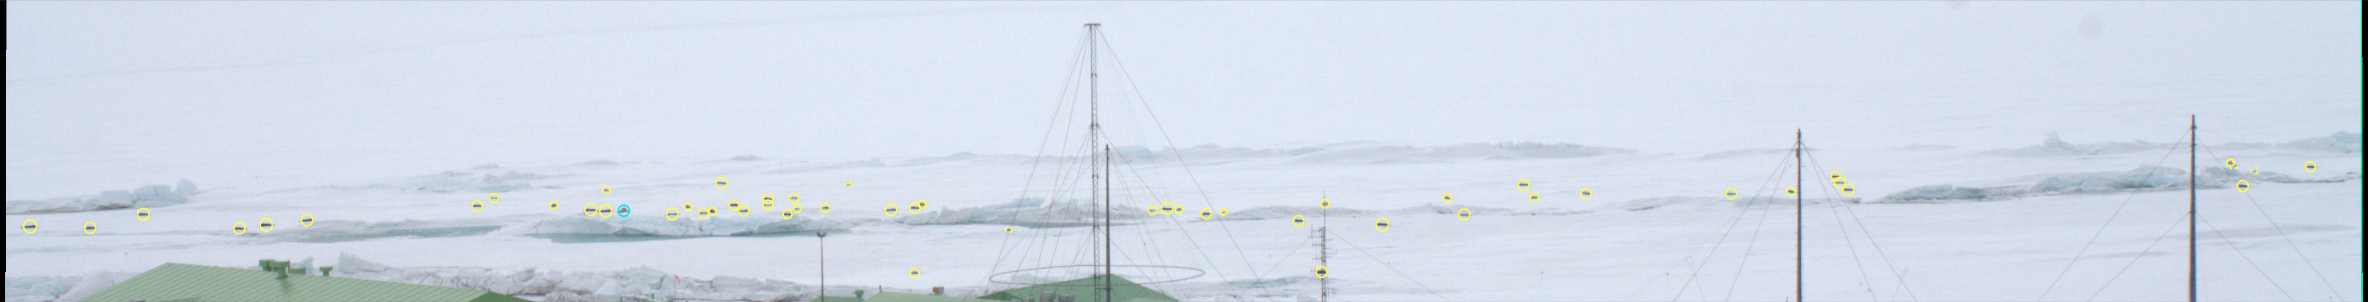
\includegraphics[width=1.0\linewidth]{figures/annotation/screenshots/cam_b.png}
  \caption{}
\end{subfigure}



\caption{ }
\label {fig:weddell_images}
\end{figure*}



\section{Discussion}


\subsection{Number of instances}
\label{sec:instances_discussion}

The instance distribution in each image has clear implications for verification based image annotation. Verifying several instances at once can be more efficient than one at a time, but verifying too many instances concurrently increases cognitive load (the very problem human in the loop machine learning seeks to address). 

Despite the ability to zoom into a small part of an image, in order to submit an image the user must review the whole image or remember which parts have been checked. For this reason when images become excessively large they should be split into pieces which can be easily verified without too much use of navigation.

This can be similar to a user interface for navigating search results, showing several results at once is much faster for a user to peruse than showing them one by one. However, if too many results are shown on each page results become lost in the crowd. A pair of studies found users do not look at results beyond 30 per page \cite{PunchoojitLumpapun2017, Zhou2007}.

The dual threshold approach helped in this regard by highlighting areas of uncertainty. For some datasets \emph{penguin surveys} and \emph{apples1}, \emph{apples2} the number of instances made it hard to keep track of progress when verifying the whole image. Combined with uncertain instances which are difficult to see without zooming, checking to ensure all annotations are present becomes difficult.

The dataset \emph{scott base} also suffers a little from this problem. The images are much wider than they are long, making navigation somewhat tedious and verifying the whole image much harder by having to zoom right out to check the whole image.

In future some method of marking parts of image as checked may help here.


